%% Journal of Glaciology manuscript driver.
\documentclass[review,jog]{igs}

\usepackage[utf8]{inputenc}
\usepackage{graphicx}
\usepackage{siunitx}
\usepackage{subcaption}
\captionsetup[subfigure]{justification=centering}
\usepackage{url}
\setlength{\Urlmuskip}{0mu plus 1mu}
\usepackage{float}
\usepackage{placeins}
\usepackage{array}
\usepackage{nameref}
\providecommand{\toprule}{\hline}
\providecommand{\midrule}{\hline}
\providecommand{\bottomrule}{\hline}

\graphicspath{{figures/introduction_methods/}{figures/results/}{figures/appendix/}}

\begin{document}
\def\FinalPass{1}

\title[Testing point-wise inference of basal friction]{Do surface and bed observables determine basal friction? A point-wise test in the Amundsen Sea sector}

\author[Matai and others]{Racheet MATAI,$^1$\protect\thanks{Present address:
  Lamont-Doherty Earth Observatory, Columbia University, USA}
  Jonathan KINGSLAKE,$^1$ Kirsty TINTO,$^1$ Andrew HOFFMAN,$^1$ Dave PORTER,$^1$}

\affiliation{%
$^1$Lamont-Doherty Earth Observatory, Columbia University, USA\\
Correspondence: Racheet Matai
\email{rmatai@ldeo.columbia.edu}}

\begin{frontmatter}
\maketitle
% BEGIN INLINED SOURCE: pass3_abstract.tex
\begin{abstract}
Accurate projections of ice-sheet contributions to sea-level rise are hindered by uncertainties in basal-sliding parameterizations. Although inverse methods can calibrate basal friction to reproduce observed velocities, the controls on inversion-derived friction remain poorly understood. We test whether surface, bed, and geophysical observables can define a consistent point-wise relationship with the inversion-derived basal-friction control $C$ across the Amundsen Sea sector of West Antarctica. Using a sector-wide Icepack inversion as the reference, we train multilayer perceptrons (MLPs) in ten experiments, each with a spatially separated 50~km square and surrounding buffer withheld from training and validation. Each predicted $C$ field is tested in an Icepack forward simulation against observed velocity. The two ice-product configurations improve on a spatially uniform-$C$ reference in eight of ten squares, while the combined configurations do so in nine of ten. Performance varies among locations, adding predictors does not consistently improve performance, and failures occur even where marginal and joint predictor support is high. The tested local predictors produce friction controls that improve modeled velocity in most withheld squares, but the learned relationships are not consistently successful across locations. These experiments highlight the limitations of constructing point-wise basal-friction parameterizations from these observables alone.
\end{abstract}
% END INLINED SOURCE: pass3_abstract.tex
\end{frontmatter}

% BEGIN INLINED SOURCE: pass3_body.tex
% BEGIN INLINED SOURCE: pass1_intro.tex
\section{Introduction}

Ice-sheet models are used to project sea-level rise, reconstruct past ice-sheet behavior, and investigate the physical processes governing ice-mass change, e.g.\ \citet{lecavalier2025history,nowicki2016ice}. These models contain structural uncertainty arising from incomplete representations of physical processes and parameter uncertainty arising from imperfectly constrained model parameters \citep{hebeler2008impact,recinos2023framework}. Both sources of uncertainty limit our ability to constrain probabilistic projections, especially for low-probability, high-impact outcomes \citep{kopp2017evolving}.

Basal slip is an important source of both structural and parameter uncertainty \citep{joughin2019regularized, bulthuis2019uncertainty}. Motion at the ice--bed interface can involve sliding over hard bedrock, deformation of subglacial sediment, and changes in basal water pressure, among other processes \citep{schoof2013ice,noble2020sensitivity}. Ice-sheet models generally represent these processes through a sliding law containing one or more spatially varying friction parameters \citep{weertman1964theory,schoof2005cavitation}. In an inversion, these parameters are adjusted to reduce the mismatch between modeled and observed quantities such as velocity \citep{macayeal1993tutorial}. The resulting friction field can therefore absorb unresolved basal processes, including bed roughness, till rheology, and hydrology \citep{tulaczyk2000basal,lu2023coupling}, as well as errors in geometry and differences among model formulations \citep{barnes2021transferability}. It is consequently an effective model parameter rather than a direct observation of basal conditions.

Inversion studies show that basal resistance across Antarctica is spatially heterogeneous \citep{morlighem2013inversion,zhao2018basal}. This motivates a working hypothesis: at the resolution of an ice-sheet model, the dimensionless basal-friction control $C(\mathbf{x})$ may be approximated by a point-wise function of observables evaluated at the same location,
\begin{equation}
\label{eq:functional_relationship}
C(\mathbf{x}) \approx f\!\left(\mathbf{z}(\mathbf{x})\right),
\end{equation}
where $\mathbf{z}(\mathbf{x})$ contains locally measured or inferred quantities that may influence basal resistance or serve as proxies for unresolved basal conditions. Equation~\ref{eq:functional_relationship} is a testable point-wise approximation at the model-grid scale, not a physical sliding law. We test it by fitting the relationship outside a held-out region and asking whether the predicted $C$ improves modeled velocity within that region, particularly where similar predictor values are well represented in the training data.

We divide the candidate predictors into two groups. The ice-product group describes ice geometry, its gradients, driving stress, and surface air temperature. The geophysical-product group describes bed geometry, bed--surface gradient alignment, geothermal heat flux, and gravity and magnetic anomalies. Ice thickness controls overburden pressure and normal stress at the bed, while surface slope governs driving stress; together, variations in thickness and surface elevation gradient impose systematic constraints on basal drag (\citealp{macayeal1989large}; \citealp[Sections 7.2--7.4 and 8.2]{cuffey2010physics}). Surface air temperature provides a large-scale upper thermal boundary condition that influences englacial and basal thermal state over long timescales. Where basal ice reaches the pressure-melting point, basal water pressure can reduce effective pressure and frictional resistance (\citealp[Chapters~6--7]{cuffey2010physics}; \citealp{iken1981effect,dawson2022ice}).

Geophysical factors can affect basal drag through bed topography and substrate composition. Bed gradients characterize topographic variation that can contribute to form drag, while deformable till can reduce resistance and enable sliding \citep{cuffey2010physics,tulaczyk2000basal,boulton2001sediment,hoffman2022impact}. Inferred friction can also depend on assumptions about ice rheology and subglacial hydrology \citep{rathmann2022inferred,mcarthur2023basal}.
Gravity disturbances reflect subsurface density variations associated with bedrock and sedimentary structure \citep{hackney2003geodetic}. Gravity data can therefore constrain broad bed geometry where direct measurements are sparse \citep{boghosian2015resolving,kennedy2020gravity}. Bedrock lithology can influence sediment characteristics, while deformable sediment can reduce basal resistance \citep{crompton2016correlations,boulton2001sediment}. Gravity measurements cannot resolve the thin (centimeter to meter scale) sediment layers that affect sliding, but larger density contrasts can identify sedimentary basins; such sediment bodies can influence ice-stream onset \citep{kennedy2020gravity,peters2006subglacial}. Magnetic anomalies reflect contrasts in crustal magnetization \citep{golynsky2018new}. In concert with gravity and radar data, they can help infer subglacial geology \citep{jordan2023geological} and regional thermal structure \citep{martos2017heat,reading2022antarctic}, thereby providing indirect context for basal drag. Geothermal heat flux supplies heat at the bed and can influence whether basal ice reaches the pressure-melting point. Where basal ice is at the melting point, additional heat can support basal meltwater production and thereby influence basal resistance \citep{dawson2022ice,kang2021evaluation}.

Previous studies have compared inferred basal resistance with radar, seismic,
and other observations of the subglacial environment, but have not established
a generally predictive local relationship. \citet{haris2024can} found
differences in basal shear stress among regions with distinct radar signatures
but did not identify a direct predictive relationship.
\citet{das2023quest} found no robust correlation between inferred sliding
parameters and radar-derived basal reflectivity over Thwaites Glacier, while
\citet{kyrke2017can} found only weak kilometer-scale association between basal
drag and seismic acoustic impedance along Pine Island Glacier (PIG).

These studies, together with our understanding of basal processes, suggest that
the relationship between basal conditions and basal resistance may be complex
and nonlinear, involving thermo-mechanical feedbacks, subglacial hydrology, and
spatially variable bed properties. Following the field inversion and machine
learning approach of \citet{parish2016paradigm}, we use machine learning to fit
the proposed nonlinear relationship between the selected observables and the
inversion-derived friction control $C$.

We use a multilayer perceptron (MLP) as a flexible nonlinear representation of $f$ in Eqn~\ref{eq:functional_relationship}. The point-wise architecture asks whether the values of the selected observables at a location contain enough information to determine the inversion control there without prescribing a particular functional form. Observed velocity is deliberately excluded from the predictor set. Because changing $C$ changes the modeled velocity, including velocity as an input would introduce a self-consistency problem and would make the inferred relationship depend directly on the velocity used to evaluate it.

Recent machine-learning studies in glaciology have addressed related but distinct inverse and constitutive problems. \citet{jouvet2023inversion} inverted a convolutional emulator of Stokes flow, while \citet{jouvet2023ice} and \citet{cheng2024forward} incorporated ice-flow physics into learned forward or inverse models. \citet{wang2025deep} used remote sensing and physics-informed deep learning to infer spatially varying ice-shelf rheology. These approaches use spatial structure or governing equations to reproduce ice-flow fields or solve inverse problems. Here, machine learning is used only to fit the local relationship in Eqn~\ref{eq:functional_relationship}.
% END INLINED SOURCE: pass1_intro.tex
% BEGIN INLINED SOURCE: pass2_intro_addendum.tex

We evaluate that hypothesis in ten spatially separated 50~km squares across the
Amundsen Sea sector. Each square and its surrounding buffer are excluded from
MLP training and validation. The predicted $C$ field is then used in a forward ice-flow simulation, and the resulting velocity is compared with observed velocity. All experiments use the same sector-wide reference inversion, constructed using observed velocity from the complete sector. The square experiments therefore test whether a point-wise relationship fitted elsewhere in the sector remains useful in a withheld location. We compare six predictor configurations and quantify how well the withheld predictor values are represented in the training data. We also withhold all of Pine Island Glacier in a secondary catchment-scale test. Because inversion-derived $C$ is not necessarily unique \citep{macayeal1993tutorial}, modeled velocity provides the primary evaluation, while direct agreement with the reference $C$ is treated as secondary (Appendix section~\nameref{app:target_distributions}).
% END INLINED SOURCE: pass2_intro_addendum.tex
% BEGIN INLINED SOURCE: pass1_methods.tex
\section{Methods}

The experiment links a sector-wide basal-friction inversion with spatially withheld tests of the learned relationships (Fig.~\ref{fig:method_overview}). The inversion provides the reference $C$ used to train the MLPs outside each excluded region. Predicted $C$ is then supplied to Icepack, and the resulting modeled velocity is compared with observations in the withheld region.

\begin{figure*}
\centering
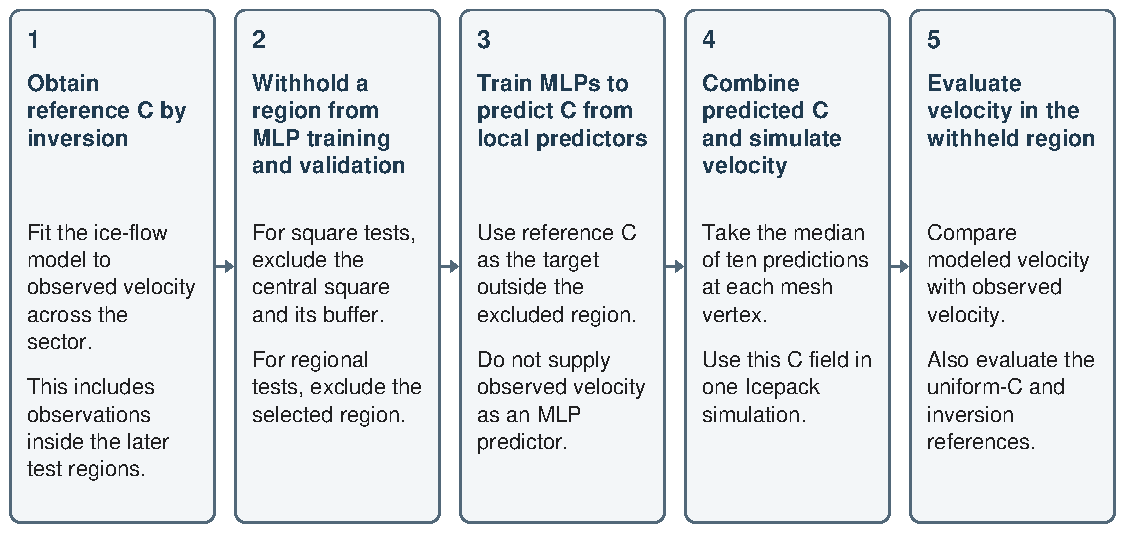
\includegraphics[width=\textwidth]{method_overview.pdf}
\caption{Steps in the spatial-transfer experiment. Each experiment--configuration pair uses one modeled velocity field obtained from the vertex-wise median of ten predicted basal-friction controls. Predicted $C$ replaces reference $C$ only within the withheld footprint or catchment, intersected with the eligible grounded area; reference $C$ is retained elsewhere. Observed velocity enters the inversion and the final velocity comparison, but is not an MLP predictor.}
\label{fig:method_overview}
\end{figure*}

\subsection{Study region and observations}

The study domain covers the Pine Island, Thwaites, and Dotson--Crosson drainage systems in the Amundsen Sea sector of West Antarctica (Fig.~\ref{fig:study_region}). The catchment outlines were delineated manually, with lateral boundaries following glacier velocity flowlines. PIG, Thwaites, and Dotson are geographic labels; they do not imply that each catchment contains one basal regime. Two non-overlapping inter-catchment corridors complete the five-region division used for regional comparisons. %Catchment membership is defined by the catchment meshes. Where meshes overlap, a location is assigned to the catchment in which it lies farthest from the boundary.

\begin{figure*}
\centering
\begin{subfigure}[t]{0.545\textwidth}
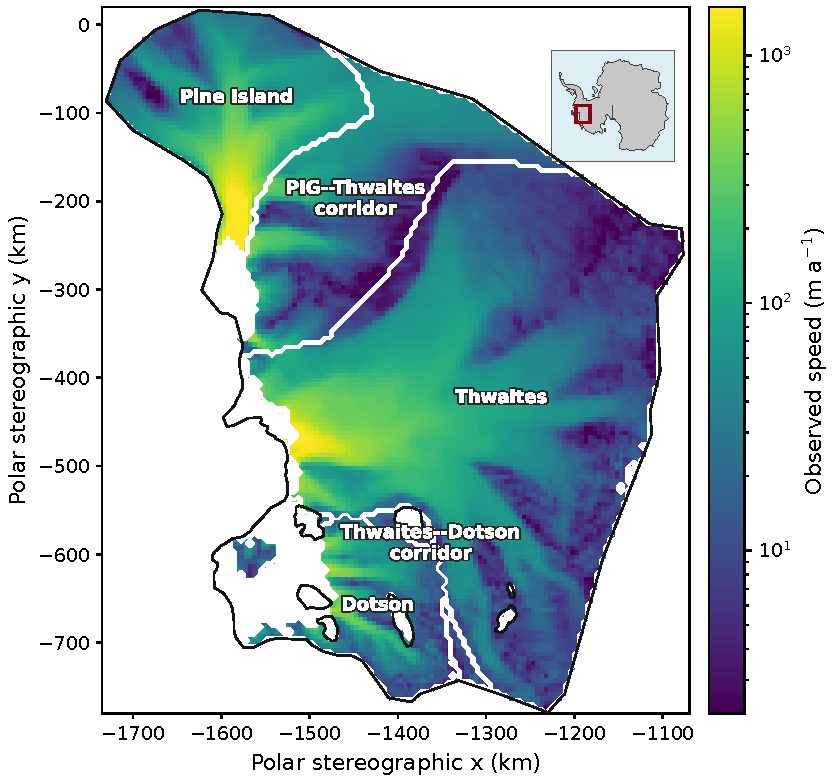
\includegraphics[width=\linewidth]{figure1a_observed_speed_and_regions.pdf}
\caption{Observed speed and regional partition.}
\end{subfigure}\hfill
\begin{subfigure}[t]{0.445\textwidth}
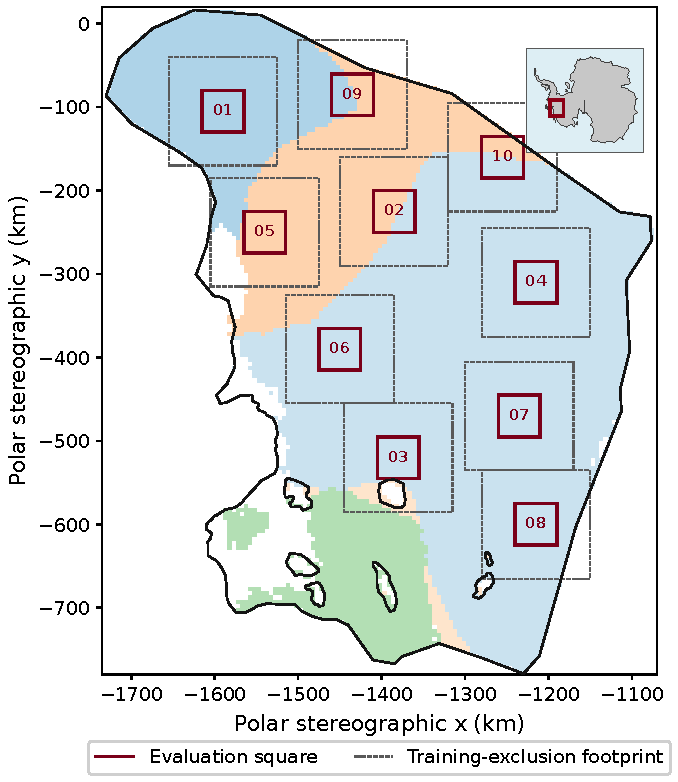
\includegraphics[width=\linewidth]{figure1b_holdout_geometry.pdf}
\caption{Primary squares and excluded footprints.}
\end{subfigure}
\caption{Study region and experimental geometry. Panel (a) shows observed MEaSUREs speed over the eligible part of the Amundsen Sea sector, with the PIG, Thwaites, and Dotson regions and the two inter-catchment corridors. Panel (b) shows the ten 50~km primary evaluation squares (solid) and their 130~km excluded footprints (dashed). Each footprint includes a 40~km buffer on every side of the central square and is excluded from MLP training and validation.}
\label{fig:study_region}
\end{figure*}

Velocity is taken from the Making Earth System Data Records for Use in Research Environments (MEaSUREs) Phase-Based Antarctica Ice Velocity Map, derived from satellite radar interferometry \citep{https://doi.org/10.5067/pz3nj5rxrh10}. Surface elevation, ice thickness and bed elevation are taken from BedMachine Antarctica, version~2 \citep{https://doi.org/10.5067/e1ql9hfq7a8m,morlighem2020bedmachine}. BedMachine combines direct observations with reconstruction that uses ice velocity in some regions. The ice-product predictors therefore
represent available geometry products, some of which already incorporate
velocity information, although velocity itself is not used as a predictor. BedMachine uses different methods to reconstruct ice thickness between
observations. Most of our test regions (detailed in following sections) lie in regions mapped
using streamline-diffusion interpolation, which favors smoother
thickness variations along flow than across flow
\citep{morlighem2020bedmachine}.

Surface air temperature and geothermal heat flux follow the products distributed with Quantarctica \citep{matsuoka2018quantarctica,comiso2000variability,an2015temperature}. Magnetic anomaly is taken from the 5~km EPSG:3031 ADMAP-2S grid \citep{eagles2024admap}, and gravity disturbance from the oriented EPSG:3031 AntGG2021 gravity-anomaly grid \citep{scheinert2024antgg}. %NetCDF and GeoTIFF products are sampled at raster cell centers before interpolation to the finite-element mesh. 
Interpolation to the model grid does not add spatial information beyond that contained in the original products, whose native resolutions and processing differ.

\subsection{Ice-flow model and basal-friction inversion}

All simulations were performed with Icepack \citep{shapero2021icepack}, using a depth-integrated stress balance based on the Shallow Shelf Approximation (SSA) \citep{macayeal1989large}. The shallow-shelf approximation neglects vertical shear, so the modeled horizontal velocity is compared directly with the observed surface velocity. Because the inferred basal-friction control depends on the adopted stress-balance approximation and basal law, the model parameter $C_b$ is model-dependent rather than a unique representation of basal conditions.

Basal friction is represented with a Weertman-type law,
\begin{equation}
\label{eq:weertman}
\boldsymbol{\tau}_b=-C_b\,\lVert\mathbf{u}\rVert^{1/n-1}\mathbf{u},
\end{equation}
where $\boldsymbol{\tau}_b$ is the resisting basal shear stress on the ice, $\mathbf{u}$ is depth-averaged horizontal velocity, $n=3$ is the exponent used in the basal law, and $C_b$ is a dimensional basal-friction coefficient with units MPa~(m~a$^{-1}$)$^{-1/3}$. A Weertman law is a simplified hard-bed parameterization and does not explicitly represent processes such as effective-pressure dependence, cavitation, or deforming till. We hold the basal law fixed so that the experiment tests the proposed mapping with one consistent ice-flow model.

Observed velocities are prescribed along the non-terminus boundaries, while an ocean-pressure traction condition is applied at the termini. Positivity and the grounding transition are imposed through
\begin{equation}
\label{eq:friction_parameterization}
C_b=\phi C_0 e^{C},
\end{equation}
where $C$ is the dimensionless inversion control used to represent spatial variation in basal friction and $C_0=0.01$~MPa~(m~a$^{-1}$)$^{-1/3}$. $\phi$ is a height-above-flotation ramp that continuously reduces basal resistance as flotation is approached and enforces $C_b=0$ over floating ice \citep{leguy2014parameterization,seroussi2014hydrostatic}. The full stress balance and grounding transition are described in Appendix section~\nameref{app:ssa}. 

%Thus, the MLP predicts $C$, while the dimensional coefficient entering the stress balance is $C_b$.

The inversion minimizes the total objective function
\begin{equation}
\label{eq:objective}
J(\mathbf{u},C;r_C)=\frac{1}{2N}\sum_{i=1}^{N}\left\lVert\mathbf{u}(\mathbf{x}_i)-\mathbf{u}_{\mathrm{obs}}(\mathbf{x}_i)\right\rVert^2+
\frac{1}{2|\Omega|}\left(\frac{L}{r_C}\right)^2\int_{\Omega}\lVert\nabla C\rVert^2\,\mathrm{d}A,
\end{equation}
where $N$ is the number of paired-velocity observations, $|\Omega|$ is the domain area, $L=7.5$~km a fixed reference  length, and $r_C$ controls smoothness. Smaller $r_C$ gives stronger smoothing. Following the use of L-curves in ice-sheet inverse models
\citep{wolovick2023regularization}, we selected
$r_C \simeq 0.014$ using a maximum-curvature criterion
(Appendix Fig.~\ref{fig:lcurve}). Gradients of Eqn~\ref{eq:objective} are obtained with the adjoint method. The resulting field (Fig.~\ref{fig:definitive_inversion}) is used for every learning experiment. 

%Following the use of L-curves in ice-sheet inverse models \citep{wolovick2023regularization}, a maximum-curvature criterion selected $r_C\simeq0.014$ from the refined candidates. The adjacent candidate $r_C\simeq0.017$ had curvature within approximately 4\% of the selected value, so the curve identifies a narrow elbow range rather than one exact value. The sector-wide inversion began from exactly $C=0$ and reached a stable endpoint after 300 optimization iterations.

\begin{figure*}
\centering
\begin{subfigure}[t]{0.32\textwidth}
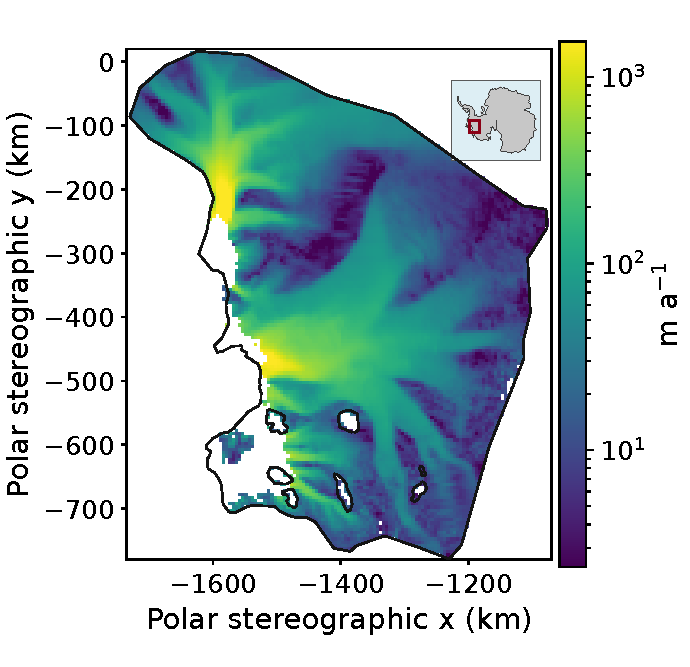
\includegraphics[width=\linewidth]{figure3a_observed_speed.pdf}
\caption{Observed speed.}
\end{subfigure}\hfill
\begin{subfigure}[t]{0.32\textwidth}
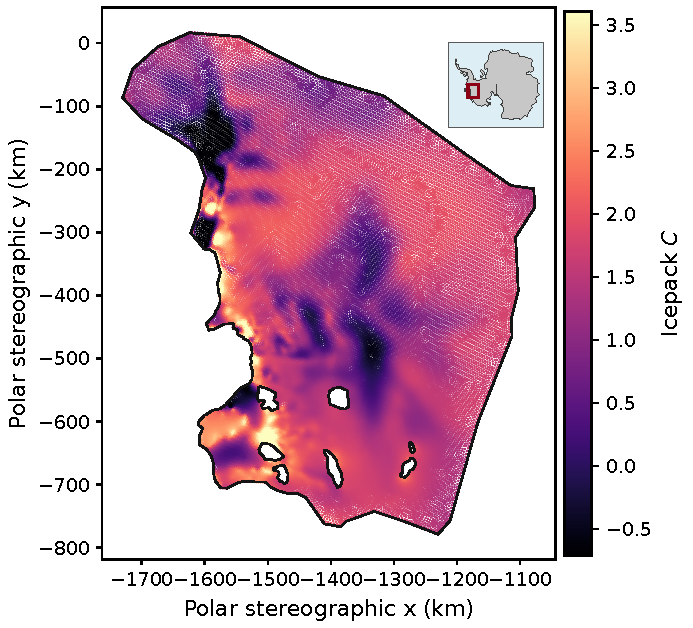
\includegraphics[width=\linewidth]{figure3b_inversion_reference_c.pdf}
\caption{Inversion-reference $C$.}
\end{subfigure}\hfill
\begin{subfigure}[t]{0.32\textwidth}
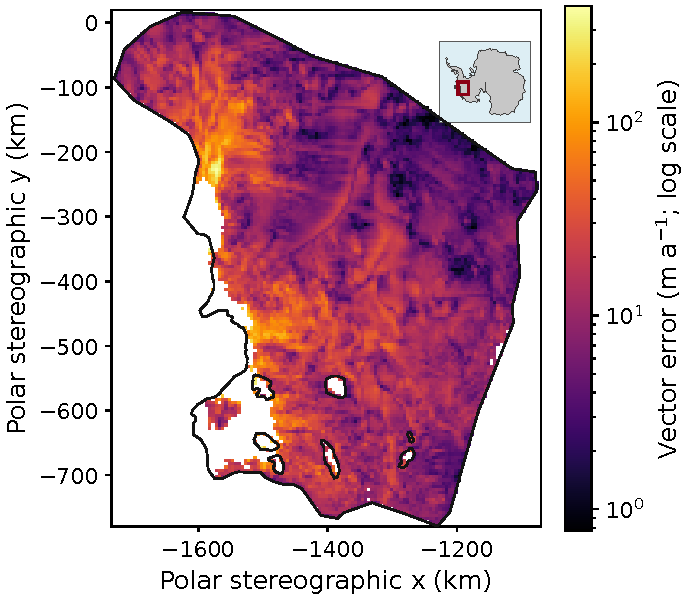
\includegraphics[width=\linewidth]{figure3c_inversion_velocity_residual.pdf}
\caption{Velocity-vector residual.}
\end{subfigure}
\caption{Sector-wide inversion used to construct the learning target. The inversion field is one regularized solution for the stated data, model equations, sliding law, boundary conditions, and regularization, and provides the reference $C$ for the learning experiments. The black line is the model-domain boundary.}
\label{fig:definitive_inversion}
\end{figure*}

\subsection{Learning dataset and predictor configurations}

We construct a common learning dataset by collocating the mesh-interpolated predictors with the inversion-reference $C$ on the observation grid. Each row contains the predictors and reference $C$ at one observation-grid location. Eligible rows are required to have finite values for all twelve predictors and both velocity components, with $\phi>0.1$ to exclude floating ice and the immediate grounding transition. The same eligibility criteria are used for all predictor configurations and experiments. Observed velocity is not included as a predictor; the twelve predictors and their six configurations (CFG01--CFG06) are summarized in Table~\ref{tab:configurations}. Gradient construction and exact row counts are given in Appendix section~\nameref{app:predictor_population}.
 
The additional predictor in CFG06 measures bed--surface gradient alignment,
\begin{equation}
\label{eq:alignment}
a_{bs}=
\frac{\nabla b\cdot\nabla s}
{\sqrt{\left(\lVert\nabla b\rVert^2+\epsilon_b^2\right)
\left(\lVert\nabla s\rVert^2+\epsilon_s^2\right)}},
\end{equation}
where $\epsilon_b=5.4\times10^{-3}$ and
$\epsilon_s=1.5\times10^{-4}$~m~m$^{-1}$. When both gradients are large
relative to these values, $a_{bs}$ approaches $\cos\theta_{bs}$. The added terms prevent the alignment from becoming unstable where either gradient is very small. This predictor describes relative alignment
without using velocity direction. The choice of $\epsilon_b$ and $\epsilon_s$
is described in Appendix section~\nameref{app:predictor_population}.

\begin{table*}
\caption{Predictors in the six configurations. Ice-product predictors are denoted I and geophysical-product predictors G. A filled circle indicates inclusion.}
\label{tab:configurations}
\centering
\ifdefined\FinalPass\tiny\setlength{\tabcolsep}{3pt}\else\scriptsize\fi
\begin{tabular}{llllcccccc}
\toprule
Symbol & Predictor & Unit & Group & CFG01 & CFG02 & CFG03 & CFG04 & CFG05 & CFG06\\
\midrule
$s$ & surface elevation & m & I & $\bullet$ & $\bullet$ & & & $\bullet$ & $\bullet$\\
$h$ & ice thickness & m & I & $\bullet$ & $\bullet$ & & & $\bullet$ & $\bullet$\\
$\lVert\nabla s\rVert$ & surface-gradient magnitude & 1 & I & $\bullet$ & $\bullet$ & & & $\bullet$ & $\bullet$\\
$\lVert\nabla h\rVert$ & thickness-gradient magnitude & 1 & I & $\bullet$ & $\bullet$ & & & $\bullet$ & $\bullet$\\
$\tau_d$ & driving stress & MPa & I & $\bullet$ & & & & &\\
$T_s$ & surface air temperature & $^\circ$C & I & $\bullet$ & $\bullet$ & & & $\bullet$ & $\bullet$\\
$b$ & bed elevation & m & G & & & $\bullet$ & $\bullet$ & $\bullet$ & $\bullet$\\
$\lVert\nabla b\rVert$ & bed-gradient magnitude & 1 & G & & & $\bullet$ & $\bullet$ & $\bullet$ & $\bullet$\\
$Q_b$ & geothermal heat flux & mW~m$^{-2}$ & G & & & $\bullet$ & $\bullet$ & $\bullet$ & $\bullet$\\
$g_d$ & gravity disturbance & mGal & G & & & $\bullet$ & & &\\
$m_a$ & magnetic anomaly & nT & G & & & $\bullet$ & & &\\
$a_{bs}$ & bed--surface gradient alignment & 1 & G & & & & & & $\bullet$\\
\bottomrule
\end{tabular}
\end{table*}

CFG01 contains all ice-product predictors and CFG02 the selected ice-product subset. CFG03 contains all geophysical-product predictors and CFG04 the selected geophysical-product subset. CFG05 combines the two selected subsets, and CFG06 adds Eqn~\ref{eq:alignment}. The subsets used in CFG02 and CFG04 were selected from preliminary catchment-scale analyses of modeled velocity conducted before the present spatially withheld experiments and were not modified based on the square results.

\subsection{Spatially withheld square experiments and predictor support}

The primary experiment uses ten 50~km squares distributed across the study
region (Fig.~\ref{fig:study_region}b). For each square, the complete 130~km
footprint is excluded from MLP training and validation, leaving a 40~km buffer
on every side of the central evaluation square. The ten excluded footprints do
not overlap. Following the rationale of spatially separated evaluation \citep{roberts2017crossvalidation,valavi2019blockcv}, the buffer reduces dependence on nearby spatially correlated training rows. It does not remove the
dependence introduced by the common sector-wide inversion or by non-local ice
flow. The central 50~km square is the primary evaluation area; the surrounding
buffer and complete footprint are used only for maps and secondary summaries,
not as additional independent tests. The quantitative basis for the buffer is
given in Appendix section~\nameref{app:buffer}.

Candidate square locations were selected using spatial separation and
predictor-support criteria so that the withheld predictor values were generally
well represented in the remaining training region. Support was assessed using
both marginal and joint criteria. No criterion based on the inversion-reference $C$ or modeled velocity errors was used in square selection. The
distribution of inversion-reference $C$ was examined only afterward because the reference field is one regularized, non-unique inversion solution, and a different predicted $C$ may still reproduce the observed velocity.
Modeled velocity errors were excluded to avoid selecting held-out regions based on how well the model ultimately performed.

Marginal support requires every included predictor at a held-out point to lie
within the 1st--99th percentile range of the corresponding eligible non-held-out
rows. Joint support asks whether the complete predictor combination has a
sufficiently close analogue in the remaining training region. We report the area fraction satisfying both criteria and retain every held-out point in the modeled velocity evaluation regardless of support. Details of the joint-support
transformation and distance threshold are given in Appendix section~\nameref{app:predictor_population}. A separate regional experiment withholds the two inter-catchment corridors and is reported in Appendix section~\nameref{app:target_distributions}.

\subsubsection{Catchment-scale transfer test}

In addition to the ten compact spatial tests, we retained Pine Island
Glacier (PIG) as one catchment-scale transfer test chosen before its results were examined. This tests whether a point-wise relationship
learned elsewhere in the Amundsen Sea sector can be transferred across an
entire glacier catchment. All eligible PIG rows were excluded
from MLP training and validation, while the remaining grounded sector,
including Thwaites, Dotson--Crosson, and the two inter-catchment corridors,
provided the training and validation rows. Predictor support in PIG was evaluated using the same marginal and joint
criteria as the square experiments and without using the inversion control
or velocity errors. 

\subsection{Model fitting and repeated realizations}

A point-wise regression model provides a direct way to test whether the
inversion-derived friction control can be expressed as a local function of the
available predictors, without introducing additional spatial information from
neighboring locations. We use a MLP as a
flexible nonlinear representation of $f(\cdot)$ in
Eqn~\ref{eq:functional_relationship}. More spatially structured architectures,
such as convolutional or graph neural networks, could use information from
neighboring locations, but would test a different hypothesis from the local
relationship considered here.

The MLP contains ten hidden layers of 200 units and predicts the
inversion-reference $C$ from the selected predictor configuration. Inputs and
targets are robustly scaled using medians and interquartile ranges calculated
from the training rows only. The network architecture, optimization settings,
model-selection procedure, and training and validation histories are given in Appendix
section~\nameref{app:training_campaign}.

For each square experiment, the eligible rows remaining after removal of the
excluded footprint are divided reproducibly into 90\% for training and 10\%
for validation. Nearby training and validation rows are not statistically
independent because of interpolation, predictor resolution, spatial
autocorrelation, and regularization of the inversion-reference field. The
random split is therefore used only for model fitting and selection, while
performance is evaluated separately in the spatially withheld central square.
Exact row counts are given in Appendix
section~\nameref{app:predictor_population}.

For each experiment and predictor configuration, we train ten reproducible
realizations that differ in the training/validation split, initial weights, and
epoch shuffling. Using multiple realizations reduces sensitivity to any one
set of training choices and provides a more stable estimate of the predicted
$C$ field. Matching realizations use the same row split across predictor
configurations to support direct comparison. The spread among realizations
reflects sensitivity to these training choices rather than calibrated predictive
uncertainty or independent spatial variability. The primary prediction is the
vertex-wise median of the ten predicted $C$ fields, which is then evaluated in
a separate Icepack forward simulation.

\subsection{Forward simulations and measures of performance}

For each experiment and predictor configuration, the vertex-wise median of
the ten predicted $C$ fields is evaluated in a separate Icepack forward
simulation. For each square, predicted $C$ replaces the inversion-reference
$C$ only within the complete 130~km excluded footprint, intersected with the
common eligible grounded mask. The inversion-reference $C$ is retained
everywhere outside that footprint. The corresponding uniform-$C$ simulation
uses the identical replacement mask, so the two simulations differ only in
the spatial pattern of $C$ inside the excluded footprint. The PIG experiment
uses the same procedure over the withheld catchment. This controlled
evaluation comprises 60 square simulations using predicted $C$, one PIG
simulation using predicted $C$, ten square-specific uniform-$C$ simulations,
and one PIG uniform-$C$ simulation.

The primary measure of performance is vector velocity RMSE (hereafter velocity RMSE) against the original paired MEaSUREs velocity components at their regular 450~m pixel centres over the evaluation area $A$. Modeled velocity is evaluated at the same locations. This evaluation is distinct from the mesh-interpolated observation field used by the solver for inversion and boundary conditions. The spatial average below is approximated using the mean squared vector residual at these equally spaced points (Appendix section~\nameref{app:training_campaign}):
\begin{equation}
\label{eq:vector_rmse}
\mathrm{RMSE}_{u}=
\left[
\frac{
\int_A
\lVert\mathbf{u}_{\mathrm{ML}}-\mathbf{u}_{\mathrm{obs}}\rVert^2
\,\mathrm{d}A
}{
\int_A \mathrm{d}A
}
\right]^{1/2}.
\end{equation}

For the maps, we also use the local vector-error magnitude
\[
e(\mathbf{x}) =
\left\|\mathbf{u}(\mathbf{x})-\mathbf{u}_{\mathrm{obs}}(\mathbf{x})\right\|.
\]

The spatially uniform-$C$ reference provides a predictor-free baseline
analogous to a mean-only model. It uses a single control value equal to the
finite-element-area-weighted mean inversion-reference $C$ over the eligible
non-held-out region. For squared error in $C$, this mean is the best-fitting
constant over that region, while containing no predictor-dependent spatial
variation. Because $C_b\propto\exp(C)$, averaging $C$ corresponds to a
geometric mean of $C_0\exp(C)$ before multiplication by the grounding ramp
$\phi$. The constant is not fitted to held-out velocity and is applied over
the same withheld replacement region as the predicted field, while the
inversion-reference $C$ is retained outside that region in both simulations.
The comparison therefore asks whether spatial variation in $C$ inferred from the predictors improves modeled velocity beyond what is obtained from a single representative friction control. We also report relative RMSE,
$\mathrm{RMSE}_{\mathrm{ML}}/\mathrm{RMSE}_{\mathrm{uniform}}$; values below
one indicate improvement over the uniform-$C$ reference.

The ten held-out squares are the independent spatial tests. For each predictor
configuration, performance is summarized by the median and interquartile range
of the ten square RMSE values. Related configurations are also compared
square by square to determine whether adding or removing predictors gives a
consistent improvement across locations.
% END INLINED SOURCE: pass1_methods.tex
% BEGIN INLINED SOURCE: pass1_results.tex
\section{Results and Discussion}

\subsection{Modeled velocity performance}

\begin{figure*}
\centering
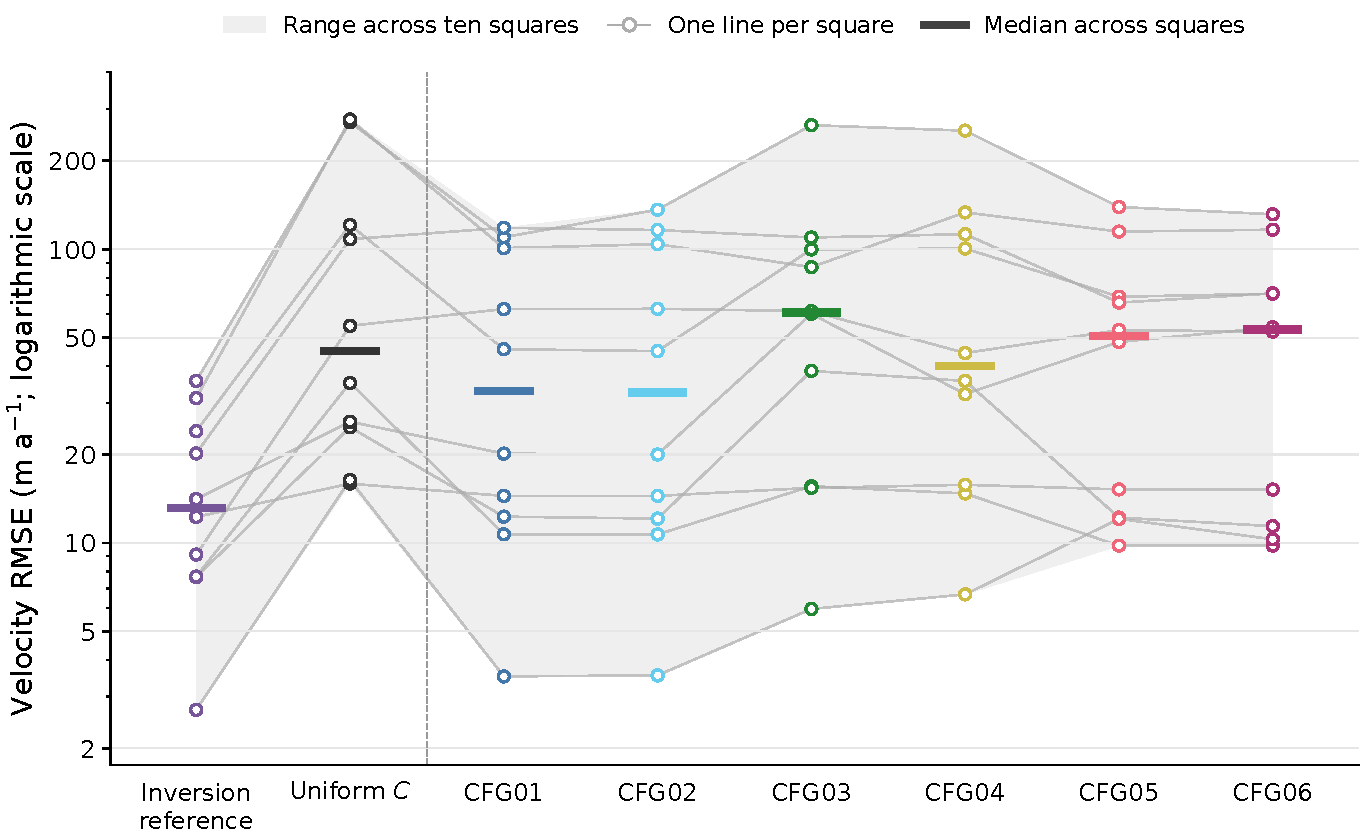
\includegraphics[width=0.75\textwidth]{figure3_square_velocity_rmse.pdf}
\caption{Velocity RMSE against observed MEaSUREs velocity in the ten central
squares. The inversion reference and square-specific uniform-$C$ reference are
followed by forward simulations using the median predicted $C$ for all six
configurations. Each gray line connects the same square; shading spans the
minimum to maximum across squares, and short horizontal marks show the medians.
The vertical axis is logarithmic. Uniform $C$ is calculated separately from
the eligible region outside each excluded footprint; both the predicted and
uniform controls replace the inversion reference only inside that footprint.
The inversion reference was fitted using sector-wide
observations, including those in the test squares.}
\label{fig:performance}
\end{figure*}

The local observables often produce a $C$ that improves modeled velocity
relative to the spatially uniform-$C$ reference, but performance varies
substantially among locations. Figure~\ref{fig:performance} shows the velocity
RMSE for each held-out square, including the inversion and uniform-$C$
references. The two ice-product configurations have the lowest median RMSE
values across the squares, 32.9~m~a$^{-1}$ for CFG01 and
32.5~m~a$^{-1}$ for CFG02, and each improves on uniform $C$ in eight of ten
squares (Table~\ref{tab:performance_summary}). CFG05 and CFG06, which combine the selected ice-product and geophysical-product
predictors, improve on uniform $C$ in nine squares, while CFG03 and CFG04, the
all- and selected-geophysical configurations, improve on uniform $C$ in six and
seven squares, respectively.

The inversion-reference solution has a substantially lower median RMSE of
13.2~m~a$^{-1}$. This is not a withheld benchmark, because the inversion was
fitted using velocity observations from the complete sector, including the
evaluation squares. It nevertheless provides context for the velocity fit
obtained with the spatially resolved inversion. The substantially larger errors
from the predicted $C$ fields show that the point-wise mappings recover only
part of the improvement available from the inversion-derived spatial structure.
At the same time, their frequent improvement over uniform $C$ shows that the
predictors contain information relevant to the effective friction control.

\begin{table*}
\caption{Velocity RMSE against observed MEaSUREs velocity in the ten central
squares. Values are the median and interquartile range across squares.
Relative RMSE uses the corresponding square-specific uniform-$C$ reference. The inversion reference was fitted using sector-wide observations,
including those inside the test squares, and therefore represents the fitted
reference rather than a withheld prediction. RMSE is in
$\mathrm{m\,a^{-1}}$.}
\label{tab:performance_summary}
\centering\small
\ifdefined\FinalPass\setlength{\tabcolsep}{4pt}\fi
\begin{tabular}{llrrrrr}
\toprule
Control/config. & Predictors & \shortstack{Median\\RMSE} & IQR & \shortstack{Better than\\uniform} & \shortstack{Median\\relative RMSE} & \shortstack{Relative RMSE\\IQR}\\
\midrule
Uniform $C$ & spatially uniform & 44.9 & 25.0--117.8 &
-- & 1.00 & 1.00--1.00\\
Inversion reference & -- & 13.2 & 8.0--23.0 &
10/10 & 0.19 & 0.17--0.29\\
\midrule
CFG01 & all ice & 32.9 & 12.8--91.3 &
8/10 & 0.45 & 0.37--0.88\\
CFG02 & selected ice & 32.5 & 12.7--93.7 &
8/10 & 0.50 & 0.37--0.87\\
CFG03 & all geophysical & 60.9 & 21.3--96.6 &
6/10 & 0.97 & 0.54--1.09\\
CFG04 & selected geophysical & 40.0 & 19.9--109.5 &
7/10 & 0.88 & 0.56--1.03\\
CFG05 & selected combined & 50.7 & 13.0--68.1 &
9/10 & 0.59 & 0.50--0.90\\
CFG06 & combined + alignment & 53.3 & 12.4--70.7 &
9/10 & 0.61 & 0.47--0.88\\
\bottomrule
\end{tabular}
\end{table*}

Removing driving stress from CFG01 to form CFG02 changes the median velocity
RMSE only slightly, from 32.9 to 32.5~m~a$^{-1}$, and both configurations
improve on uniform $C$ in eight squares. Because driving stress is derived from
ice thickness and surface slope, which are already included in CFG02, supplying
it explicitly provides no consistent improvement across the ten squares. Among the geophysical configurations, CFG04 has a lower median velocity RMSE than CFG03 (40.0 versus 60.9~m~a$^{-1}$), but CFG04 has lower velocity RMSE than CFG03 in only five of the ten squares; CFG03 performs better in the other five. Relative to uniform $C$, CFG03 reduces velocity RMSE in six squares and CFG04 in seven.

%Their training behavior also differs: across the primary-square runs, the median validation MSE decreases by a factor of 19.4 for CFG02 but only 1.68 for CFG04 (Appendix Fig.~\ref{fig:training_convergence}). These factors describe the decrease from each configuration's initial loss and do not measure the fraction of target variation reproduced.

Combining the selected predictor groups does not produce a consistent advantage
over either group alone. CFG05 performs better than CFG02 in three squares and
better than CFG04 in seven. Adding bed--surface gradient alignment in CFG06
again divides the comparison evenly, with CFG06 performing better than CFG05
in five squares and worse in five. The paired sign tests provide no statistical
evidence of a consistent advantage in these five configuration contrasts
(Appendix section~\nameref{app:training_campaign}); this does not establish
equivalence or negate the improvements over uniform $C$. Overall, the relative
performance of the predictor configurations changes among squares, indicating
that no tested predictor set provides a uniformly successful point-wise
relationship across the study region.

\subsection{Predictor support and modeled velocity performance}

We next examine whether poor modeled velocity performance is associated with low predictor support. Across the ten primary squares, predictor support is
generally high (Fig.~\ref{fig:support_skill}a). Marginal support covers more
than 94\% of each primary square, while lower joint support is concentrated
mainly in SQ08. High support, however, does not guarantee good modeled velocity performance. Figure~\ref{fig:support_skill}b shows performance relative to uniform $C$; a relative RMSE greater than one means that the predicted control performs worse than the uniform-$C$ reference. SQ07--CFG03, for example, has 99.4\% support by both criteria but a relative RMSE of 2.33, while SQ02--CFG04 has 97.3\% support and a relative RMSE of 1.44 (Table~\ref{tab:supported_failures}). These failures cannot be explained solely by individual predictors falling outside their training ranges or by the absence of a nearby multivariable match under the adopted definition.

\begin{figure*}
\centering
\begin{subfigure}[t]{0.49\textwidth}
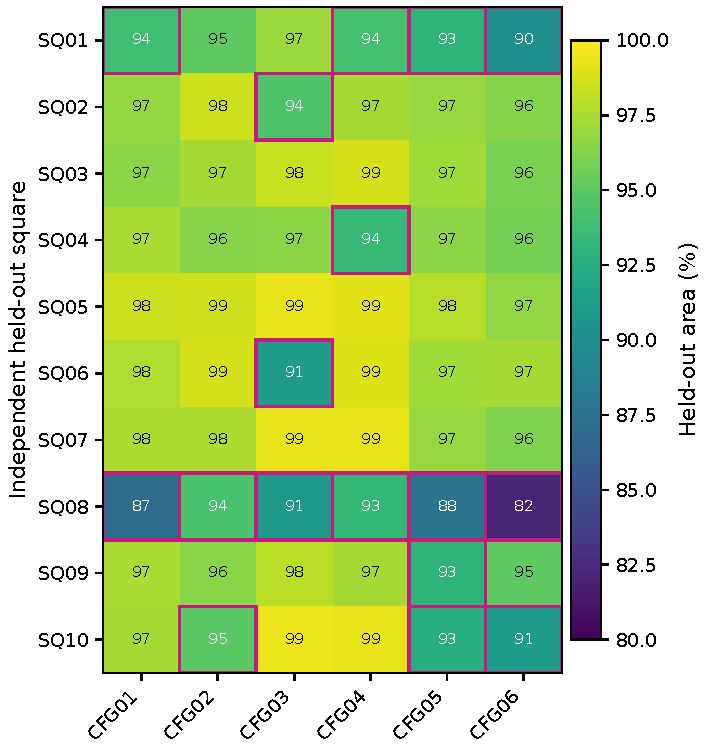
\includegraphics[width=\linewidth]{figure4a_input_support.pdf}
\caption{Area satisfying both support criteria.}
\end{subfigure}\hfill
\begin{subfigure}[t]{0.49\textwidth}
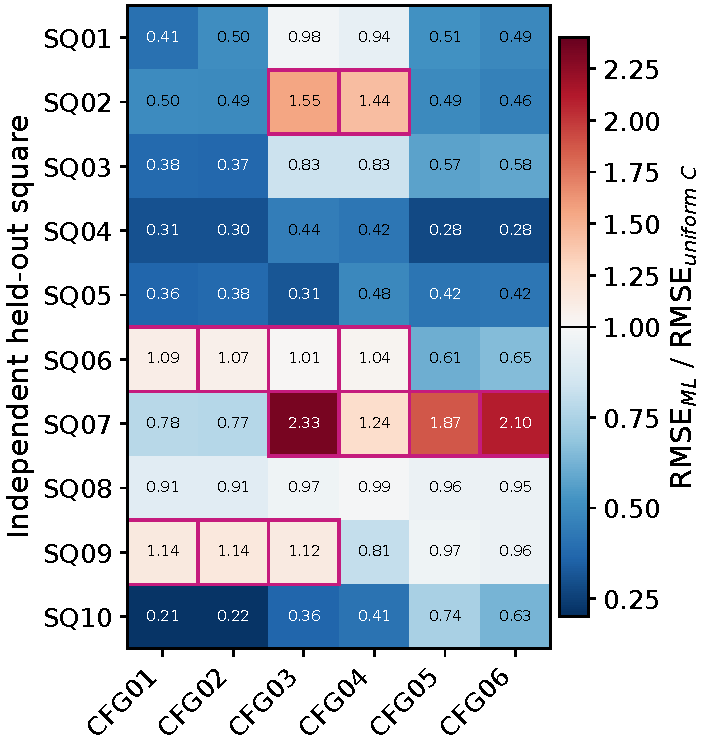
\includegraphics[width=\linewidth]{figure4b_relative_velocity_skill.pdf}
\caption{RMSE relative to uniform $C$.}
\end{subfigure}
\caption{Predictor support and modeled velocity performance in the ten spatial tests for six predictor configurations. Panel (a) gives the percentage of each held-out area satisfying both marginal and joint support; magenta outlines mark values below the 95\% criterion. Panel (b) gives relative RMSE; magenta outlines mark cases that do not improve on the spatially uniform-$C$ reference. Marginal bounds use eligible non-held-out rows, while joint matches use the 5~km reference grid within the training region.}
\label{fig:support_skill}
\end{figure*}


\begin{table}
\centering
\caption{Examples of poor performance, defined here as velocity RMSE exceeding the uniform-$C$ reference, despite high predictor support. Support is the percentage of held-out points that satisfy both the marginal and joint criteria.}
\label{tab:supported_failures}
\begin{tabular}{llrrrr}
\toprule
Square & Config. & Support (\%) & ML RMSE & Uniform RMSE & Relative RMSE\\
       &         &              & \multicolumn{2}{c}{(m~a$^{-1}$)} & \\
\midrule
SQ02 & CFG04 & 97.3 & 35.6  & 24.8  & 1.44\\
SQ06 & CFG01 & 97.6 & 118.3 & 108.2 & 1.09\\
SQ07 & CFG03 & 99.4 & 60.2  & 25.9  & 2.33\\
SQ09 & CFG02 & 96.4 & 62.7  & 54.8  & 1.14\\
\bottomrule
\end{tabular}
\end{table}


Predictor support indicates whether similar predictor combinations are represented in the training region, but does not distinguish between densely and sparsely sampled parts of predictor space. We therefore examined whether training representation was associated with errors in the predicted $C$ for CFG02 and CFG04 (Appendix section~\nameref{app:training_representation}). For CFG02, $C$ RMSE increased with sparser representation in seven of the ten squares, but the overall relationship was weak. The median within-square Spearman correlation between training-representation percentile and absolute $C$ error was only 0.069, and the median $C$ RMSE differed by only 0.004 across the three representation categories. CFG04 showed no similar pattern, with a median correlation between representation percentile and absolute $C$ error of $-0.052$. Sparse training representation is therefore associated with larger $C$ RMSE in some CFG02 experiments, but the relationship is weak and is not shared by CFG04.

Training representation also does not show a consistent correspondence with modeled velocity performance, as illustrated by the square-level examples in Appendix section~\nameref{app:training_representation}. In some squares, modeled velocity has lower RMSE than uniform $C$ in sparsely represented categories but not in better-represented categories. The same Appendix examples also show that closer agreement with the inversion-reference $C$ does not consistently correspond to lower relative RMSE. Training representation therefore does not by itself explain the failures to improve modeled velocity relative to uniform $C$.
\subsection{Spatial patterns of success and failure}

\begin{figure}
\centering
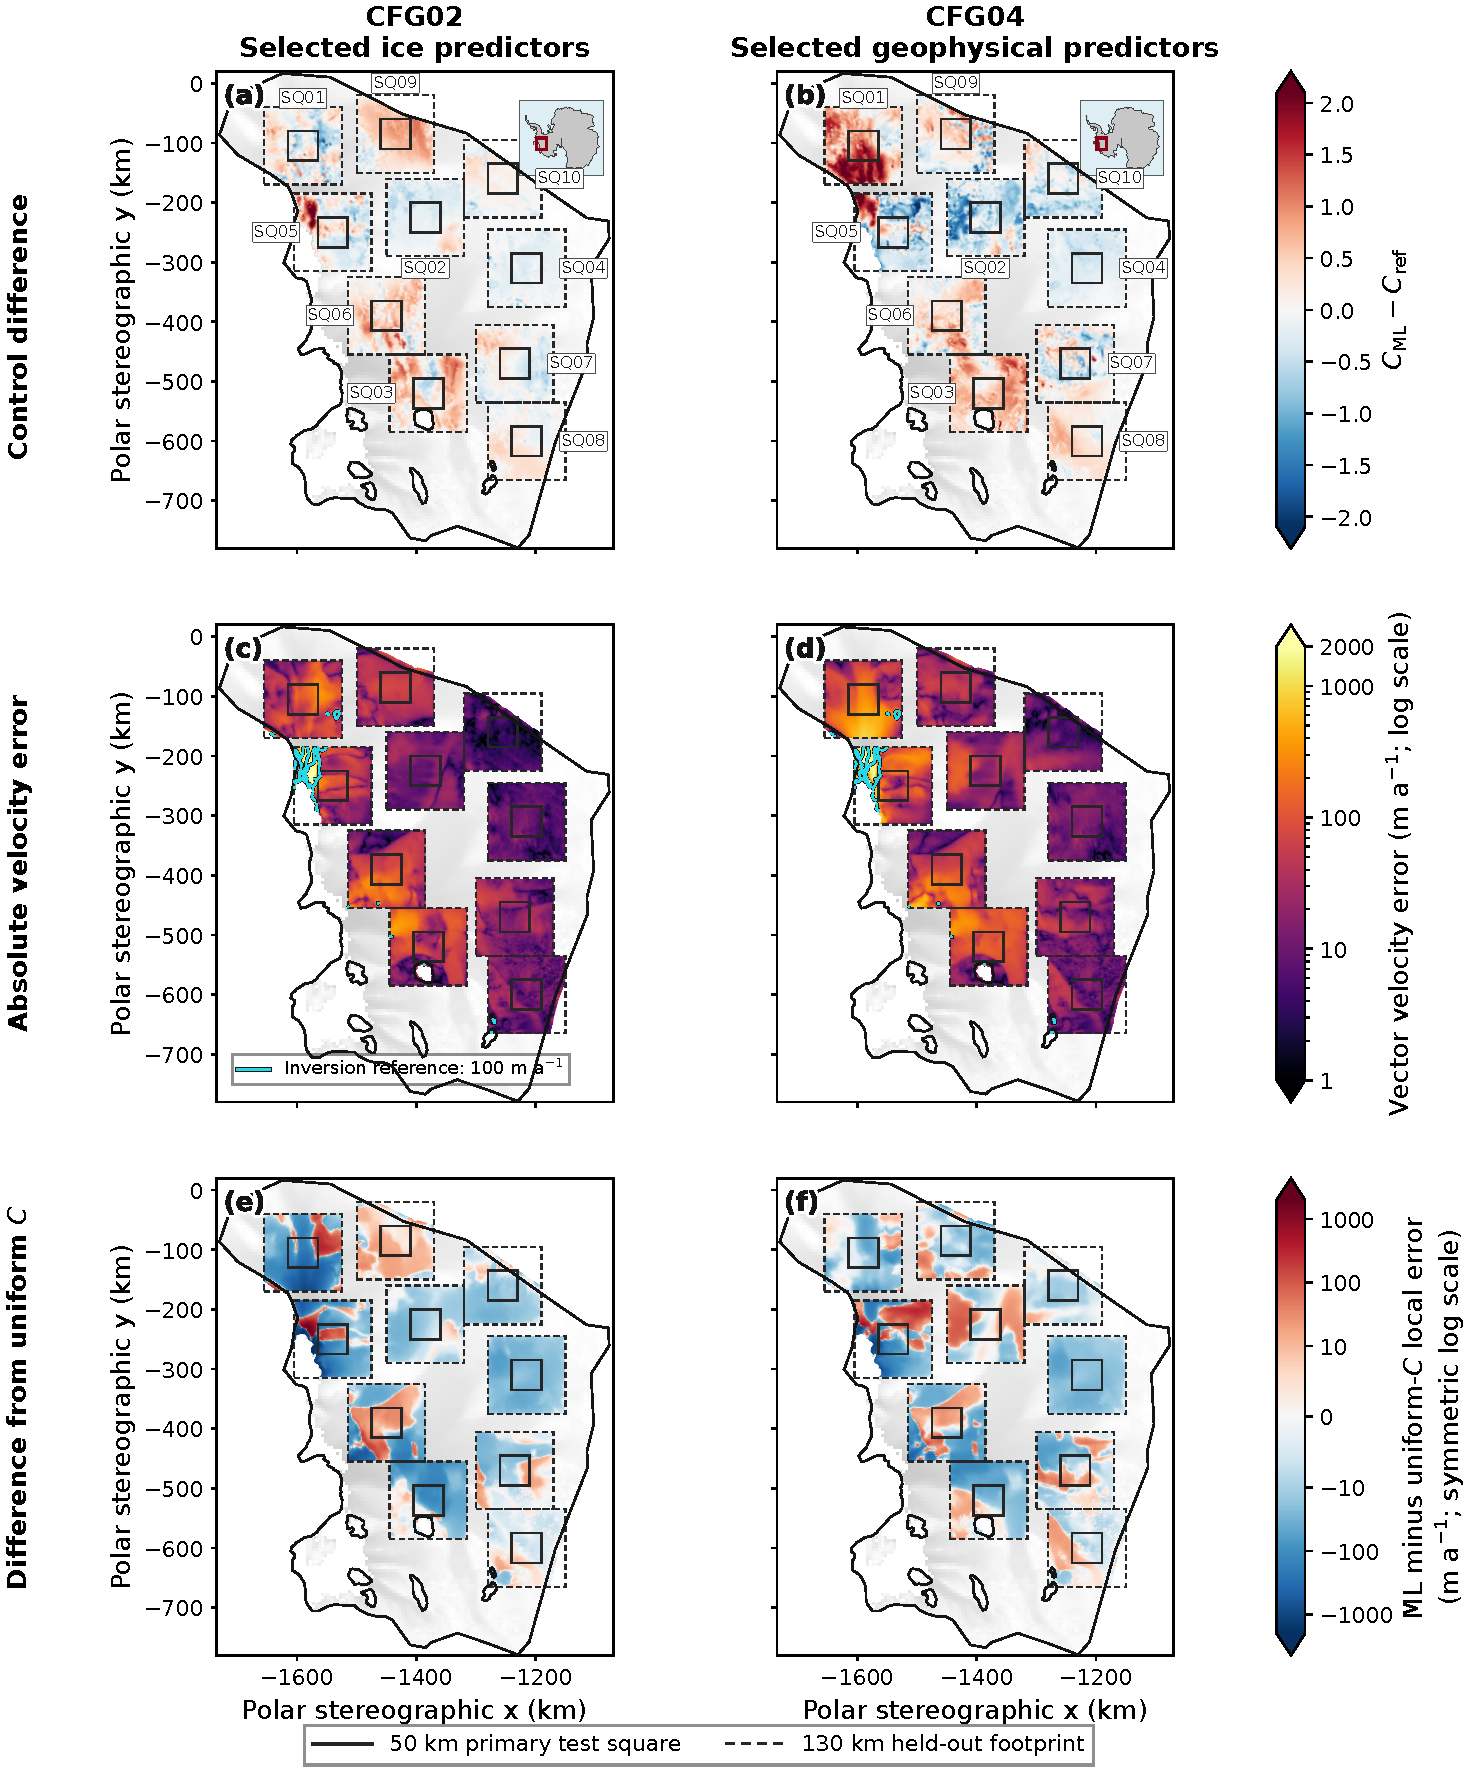
\includegraphics[width=0.97 \textwidth]{figure5_spatial_control_velocity_uniform_comparison.pdf}

\caption{Spatial comparison of the selected ice-product configuration
(CFG02; left) and selected geophysical-product configuration (CFG04; right).
Panels (a, b) show $C_{\mathrm{ML}}-C_{\mathrm{ref}}$. Panels (c, d) show the
vector velocity error relative to MEaSUREs observations,
$e_{\mathrm{ML}}=\lVert\mathbf{u}_{\mathrm{ML}}-
\mathbf{u}_{\mathrm{obs}}\rVert$. Panels (e, f) show
$e_{\mathrm{ML}}-e_{\mathrm{uniform}}$; negative values indicate lower local
error for the predicted control and positive values indicate lower error for
uniform $C$. Cyan contours in panels (c, d) mark an inversion-reference
velocity error of $100\,\mathrm{m\,a^{-1}}$. In each experiment, both controls
replace the inversion reference only inside the complete 130~km footprint.
Velocity errors use the original paired MEaSUREs components and are shown as
$1.8\,\mathrm{km}$ bin means for legibility; all statistics were calculated from the evaluated observation-grid points.}
\label{fig:square_maps}
\end{figure}

Figure~\ref{fig:square_maps} compares CFG02, the selected ice-product configuration, with CFG04, the selected geophysical-product configuration. The two ice-product configurations have nearly identical summary performance, so CFG02 is used to represent that predictor group without repeating a visually similar map. Each square comes from a separate set of MLPs for which the complete 130~km footprint was excluded from training and validation; the panels therefore assemble ten separately withheld predictions rather than one sector-wide prediction. In every simulation, the predicted and uniform controls replace the inversion reference only inside the corresponding footprint. Across the central 50~km squares, CFG02 has lower velocity RMSE than CFG04 in eight of ten tests. Over the complete 130~km footprints, both configurations improve on uniform $C$ in nine of ten tests, with median relative RMSEs of 0.64 for CFG02 and 0.86 for CFG04. Across the ten central 50~km squares, velocity error exceeds $100\,\mathrm{m\,a^{-1}}$ over 13.0\% for CFG02 and 22.8\% for CFG04, compared with only 0.13\% for the inversion-reference solution. Thus, although the predicted controls often improve on uniform $C$, regions of large absolute velocity error remain much more extensive than for the fitted inversion-reference control.  %Panels (c, d) show the absolute errors that remain, while panels (e, f) show where predicting spatial variation in $C$ reduces or increases local error relative to uniform $C$.

The maps show that the advantage of the ice-product configuration occurs
across several distinct flow settings. In the fast PIG test SQ01, the
central-square RMSE ratio is 0.50 for CFG02 and 0.94 for CFG04, with the
largest CFG02 improvement concentrated in the fast-flowing part of the
square. The local error difference adds an important distinction: CFG02
reduces error over 84.8\% of the central square, with a median pointwise
reduction of $133.5\,\mathrm{m\,a^{-1}}$, whereas CFG04 reduces error at
every evaluated point but has a much smaller median pointwise reduction of
$14.8\,\mathrm{m\,a^{-1}}$. Thus, the fraction of the square with lower local error does not by itself
determine the RMSE improvement; the magnitude and spatial distribution of the
error reductions are also important. CFG02 also gives the larger improvement in moderately fast Thwaites flow in SQ03 (0.37 versus 0.83). There, local error is lower than for uniform $C$ over 90.4\% of the central square for CFG02 and 77.5\% for CFG04. Good performance is not confined to fast flow:
both configurations improve substantially on uniform $C$ in the slow
Thwaites square SQ04 (0.30 and 0.42) and the slow PIG--Thwaites corridor
square SQ10 (0.22 and 0.41).

The large absolute residuals in the SQ05 footprint occur where it extends
from the PIG--Thwaites corridor into fast PIG flow. These large residuals
contribute disproportionately to the footprint-wide RMSE, yet both learned
controls still improve on uniform $C$ (ratios of 0.85 and 0.86).
Figure~\ref{fig:square_maps} panels (e, f) show that this footprint contains both reductions and
increases in local error: CFG02 reduces error over 80.7\% of its evaluated
area and CFG04 over 60.2\%. The large absolute errors in panels (c, d)
therefore coexist with improvements relative to the uniform control.
The inversion-reference velocity error is also elevated in this part of
SQ05, indicating that some of the mismatch remains even with the fitted
reference $C$. Over the complete footprint, however, the velocity RMSEs
are $539.5$ and $546.2\,\mathrm{m\,a^{-1}}$ for CFG02 and CFG04, compared
with $77.1\,\mathrm{m\,a^{-1}}$ for the inversion reference. The predicted
controls therefore introduce substantial additional error.

Although CFG02 performs better than CFG04 in most squares, the relative
performance of the two predictor groups varies by location. In SQ02,
which spans the PIG--Thwaites corridor and Thwaites, CFG02 performs
substantially better than the uniform-$C$ reference, whereas CFG04
performs worse. The central-square RMSE ratios are 0.49 for CFG02 and
1.44 for CFG04, and the corresponding full-footprint ratios are 0.58
and 1.91. The local comparison shows that CFG02 reduces error over
99.8\% of the central square, whereas CFG04 reduces it over only 42.5\%.
The higher CFG04 RMSE therefore accompanies a mixture of local
improvements and deteriorations, rather than uniformly larger errors.
CFG02 also agrees more closely with the inversion-reference control
in the central square, with a $C$ RMSE of 0.22 compared with 0.61 for
CFG04. SQ09, spanning PIG and the PIG--Thwaites corridor, shows the
opposite pattern: CFG04 improves on uniform $C$ while CFG02 does not,
with central-square ratios of 0.81 and 1.14 and full-footprint ratios
of 0.88 and 1.20, respectively. In this central square,
$e_{\mathrm{ML}}-e_{\mathrm{uniform}}$ is positive at every evaluated
point for CFG02 and negative at every evaluated point for CFG04.
CFG04 also has the lower central-square $C$ RMSE in SQ09
(0.49 versus 0.74). These examples show that neither predictor group
performs better at every location. The central 50~km square remains
the primary withheld-region test, while the complete 130~km footprint
is used only as a secondary spatial diagnostic.

In SQ06, both configurations are slightly worse than uniform $C$ in the
central Thwaites square (ratios of 1.07 and 1.04), despite simultaneous
predictor support exceeding 98\%. Local error is lower than uniform $C$
over only 12.6\% of the central square for CFG02 and 22.6\% for CFG04.
Over the complete footprint, however, the ratios decrease to 0.62 and
0.79, and local error reductions cover 54.1\% and 59.5\% of the evaluated
area, respectively. The difference maps therefore show how improvements
around the central square can accompany poorer performance within it.
Similarly, CFG04 changes from a ratio of 1.24 in central SQ07 to 0.80
over the complete footprint. In contrast, the CFG04 failure in SQ02
and the CFG02 failure in SQ09 remain even when the full footprints
are evaluated. SQ08 presents a different case: the uniform-$C$ error is already only 15.9~m~a$^{-1}$, compared with 12.3~m~a$^{-1}$ for the inversion-reference simulation, leaving relatively little scope for improvement. CFG02 and CFG04 give RMSE values of 14.5 and 15.8~m~a$^{-1}$, respectively. Although local error is lower than for uniform $C$ over 75.0\% and 71.3\% of the central square, the median local reductions are only $4.3$ and $5.0\,\mathrm{m\,a^{-1}}$. In this case, widespread negative values in panels (e, f) represent small absolute gains, and the larger residuals elsewhere limit the reduction in RMSE.

As discussed above, agreement with the inversion-reference $C$ and velocity performance coincide in SQ02 and SQ09. In fact, when comparing CFG02 with CFG04 within each of the ten central squares, the configuration with lower $C$ RMSE also has lower velocity RMSE. The size of the improvement in velocity RMSE from one configuration to the other, however, does not follow directly from the magnitude of the control error. Over
the complete SQ06 footprint, CFG02 and CFG04 have nearly identical
$C$ RMSE values (0.435 and 0.439), while their velocity RMSE ratios
differ substantially (0.62 and 0.79). Conversely, over the complete
SQ05 footprint, the lower $C$ RMSE of CFG02 (0.57 versus 0.85 for
CFG04) accompanies only a modest reduction in velocity RMSE
(539.5 versus $546.2\,\mathrm{m\,a^{-1}}$). Closer agreement with
the inversion-reference control therefore does not translate into a
proportional improvement in velocity RMSE. Within the individual
squares, larger absolute local differences from the inversion-reference $C$ generally coincide with larger local velocity errors, although the strength of this relationship varies among locations. The median within-square Spearman correlations are 0.32 for CFG02 and 0.42 for CFG04, indicating a modest positive association rather than a one-to-one correspondence between $C$ error and velocity error.

The spatial pattern of the control difference may help explain this
variation. Membrane stresses couple neighboring locations, so a
change in $C$ can alter velocity beyond the location where it is
applied. Local velocity error can therefore reflect control
differences elsewhere as well as those at the same point.
The sensitivity of the central-square results to the region over which $C$
is replaced is quantified in Appendix section~\nameref{app:replacement_sensitivity}.
Future
work could use spatial sensitivity analysis to examine how
perturbations to $C$ in different parts of the domain contribute to
the velocity response.

Taken together, the ten central-square tests show that the selected
ice-product and geophysical-product configurations improve velocity
RMSE relative to uniform $C$ in a majority of the squares.
Neither configuration improves every square, and some failures
persist across the complete withheld footprint despite high
predictor support. The selected predictors therefore contain information that can improve modeled velocity relative to a uniform control, but they do not define a point-wise relationship that is consistently successful across locations.

\subsection{Catchment-scale test at Pine Island Glacier}

The secondary catchment-scale experiment tests whether the point-wise relationship remains useful when all of PIG is withheld. We evaluate CFG02, the selected ice-product configuration, using the same ice-flow model and evaluation procedure as in the square experiments. The
spatially uniform-$C$ reference produces a vector velocity RMSE of
$384.9\,\mathrm{m\,a^{-1}}$, whereas CFG02 produces an RMSE of
$354.8\,\mathrm{m\,a^{-1}}$. This corresponds to a modest 8\% reduction in
RMSE relative to the uniform-$C$ reference. The inversion-reference simulation has an RMSE of $48.1\,\mathrm{m\,a^{-1}}$, showing that the transferred point-wise mapping recovers only a small fraction of the improvement obtained with the spatially resolved inversion.

\begin{figure*}[!t]
\centering
\begin{subfigure}[t]{0.32\textwidth}
\centering
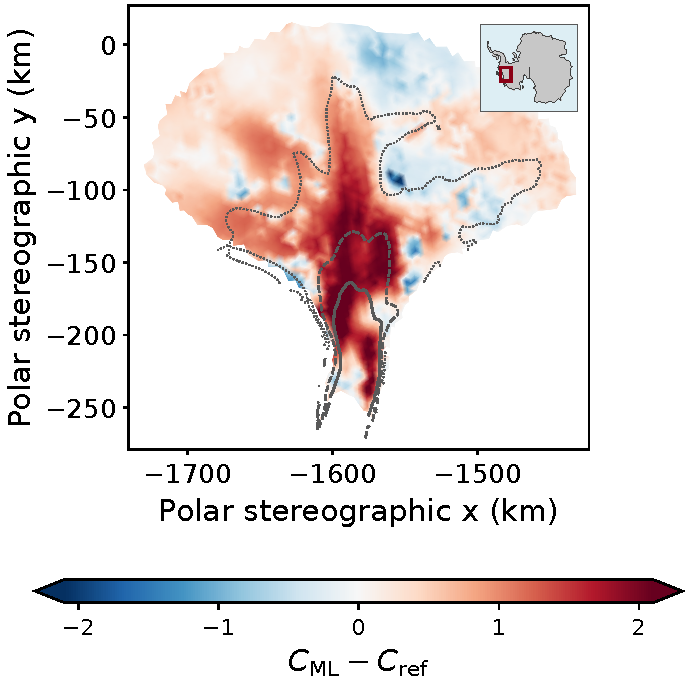
\includegraphics[width=\linewidth,keepaspectratio]
{figure6a_pig_cfg02_control_difference.pdf}
\caption{Difference from the inversion-reference control.}
\end{subfigure}
\hfill
\begin{subfigure}[t]{0.32\textwidth}
\centering
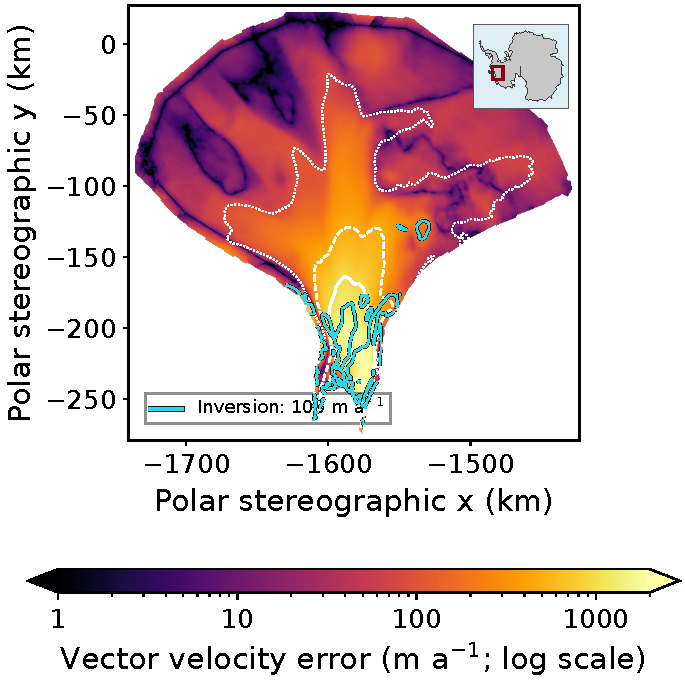
\includegraphics[width=\linewidth,keepaspectratio]
{figure6b_pig_cfg02_velocity_error.pdf}
\caption{Local velocity-vector error.}
\end{subfigure}
\hfill
\begin{subfigure}[t]{0.32\textwidth}
\centering
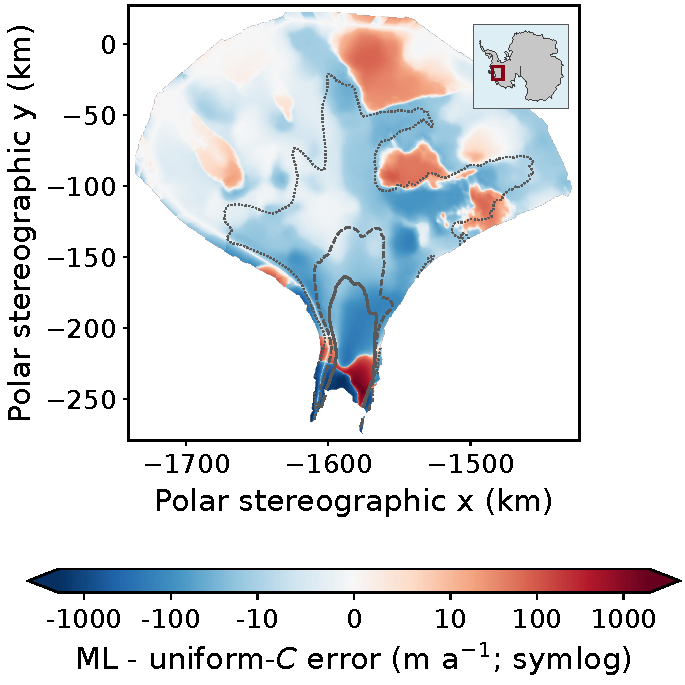
\includegraphics[width=\linewidth,keepaspectratio]
{figure6c_pig_cfg02_uniform_comparison.pdf}
\caption{Local error relative to uniform $C$.}
\end{subfigure}

\caption{Spatial evaluation of CFG02 with all of PIG withheld.
Panel (a) shows the median predicted control relative to the
inversion-reference control. Panel (b) shows
$\lVert\mathbf{u}_{\mathrm{ML}}-\mathbf{u}_{\mathrm{obs}}\rVert$.
Panel (c) shows the difference between the local CFG02 and uniform-$C$
velocity errors; negative values indicate lower error for CFG02 and positive
values indicate lower error for uniform $C$. Contours mark observed speeds
of $100$ (dotted), $500$ (dashed), and
$1000\,\mathrm{m\,a^{-1}}$ (solid). The cyan contour in panel (b) marks an
inversion-reference velocity error of $100\,\mathrm{m\,a^{-1}}$. Velocity fields are rendered from the
original $450\,\mathrm{m}$ grid using display interpolation; all
reported statistics use the original grid values. Both CFG02 and uniform
$C$ replace the inversion reference only inside the PIG holdout.}
\label{fig:pig_maps}
\end{figure*}

CFG02 lowers the local velocity error relative to uniform $C$ over 77.6\%
of the evaluated PIG area (Fig.~\ref{fig:pig_maps}). The improvement occurs
across all observed-speed classes. The relative RMSE is 0.59 below $100\,\mathrm{m\,a^{-1}}$, 0.84 between 100 and $500\,\mathrm{m\,a^{-1}}$, 0.89 between 500 and $1000\,\mathrm{m\,a^{-1}}$, and 0.96 above $1000\,\mathrm{m\,a^{-1}}$. The improvement is therefore spatially
widespread, but its influence on the catchment-wide statistic is concentrated
in fast flow. The fastest 10\% of the evaluated area, corresponding to observed speeds
above approximately $504\,\mathrm{m\,a^{-1}}$, contributes 59.8\% of the
total squared-error reduction relative to uniform $C$, but still accounts
for 89.5\% of the CFG02 squared error. In the fastest flow
($>1000\,\mathrm{m\,a^{-1}}$), the RMSE remains
$1390.0\,\mathrm{m\,a^{-1}}$, compared with
$1448.8\,\mathrm{m\,a^{-1}}$ for uniform $C$. Thus, CFG02 improves much of
the slow and intermediate-speed catchment interior and parts of the
fast-flowing trunk, but provides only a modest relative improvement in the
fastest downstream flow. This spatial concentration explains how CFG02 can
lower error across most of the catchment while retaining a large
catchment-wide RMSE.

Locations where the inversion-reference error is at least $100\,\mathrm{m\,a^{-1}}$ comprise 3.9\% of the evaluated PIG area but contain 47.1\% of the CFG02 squared error. The remaining error is not confined to those locations: most locations with CFG02 error above $100\,\mathrm{m\,a^{-1}}$ lie outside regions where the inversion-reference error exceeds $100\,\mathrm{m\,a^{-1}}$. Predictor support alone does not explain the spatial pattern. For CFG02,
marginal support covers 97.5\% of the evaluated PIG area, joint support covers
93.3\%, and 91.9\% satisfies both criteria. Of the net squared-error reduction
relative to uniform $C$, 79.8\% occurs within the area satisfying both support
criteria. CFG02 nevertheless contains both successful and unsuccessful regions
where predictor support is strong.
CFG02 has a $C$ RMSE of 0.85 across PIG. Locations with larger absolute differences from reference $C$ also tend to have larger velocity errors, with a Spearman correlation of 0.67. This indicates a relatively strong positive association and is larger than the median within-square correlation of 0.32 for CFG02. The association between training-representation percentile and absolute $C$ error is much weaker. $C$ RMSE increases from 0.742 to 0.877 and 0.898 across the three categories of progressively sparser representation, but the Spearman correlation between representation percentile and absolute $C$ error is only 0.031. This near-zero correlation indicates that having fewer nearby training examples does not correspond to a consistent increase in local $C$ error across PIG.



\subsection{Interpreting the point-wise relationship}

Taken together, the experiments separate three related questions: whether the
predictor values in a held-out region are represented in the training data,
whether the predicted $C$ resembles the reference $C$, and whether the
predicted $C$ improves modeled velocity. The results show that these questions
can have different answers. High predictor support can coexist with poor
velocity performance, and sparser training representation does not consistently
produce larger $C$ errors. Agreement with the reference $C$ is also related to,
but does not determine, the resulting velocity error. The PIG experiment shows
that the same distinctions remain important when the held-out region is
expanded from a 50~km square to an entire glacier catchment.

The spatial differences in performance are not simply explained by the
BedMachine diagnostics considered here. Reported bed-elevation uncertainty has
only a weak relationship with local velocity error across the square tests
(Appendix~\ref{app:bedmachine_diagnostics}). Comparisons among BedMachine
source classes are more limited because eight of the ten central squares
contain only streamline-diffusion cells. Nevertheless, CFG02 velocity RMSE
ranges from 3.5 to 136.3~m~a$^{-1}$ across those eight squares, showing that
differences in reconstruction class alone cannot explain the large spatial
variation in performance. Reconstruction may still matter within a source
class, for example if smoothing removes local bed variations that could help
distinguish basal settings, but the present analysis does not isolate this
effect.

More fundamentally, the available predictors may not capture all of the
physical variability relevant to $C$. For example, \citet{hoffman2022impact}
showed that small-scale basal roughness can strongly influence basal
resistance, while such scales are not resolved in continental-scale datasets.
The geophysical products also provide indirect information at relatively
coarse spatial resolution. In addition, the inferred $C$ depends on the
adopted stress balance, basal law, and regularized inversion, rather than
representing a unique physical property of the bed.

The point-wise formulation itself may also be limiting. The MLP uses only the
predictor values at each location and cannot use information from neighboring
locations. At the same time, membrane stresses couple the velocity response
across space, so changes in $C$ at one location can affect velocity elsewhere.
This is consistent with theoretical limits on local basal inference, in which
basal disturbances are filtered through spatially coupled ice flow before
appearing at the surface
\citep{gudmundsson2003transmission,raymond2005relationship,
gudmundsson2008limit}. The present experiments therefore identify several
possible explanations for the remaining errors, but do not determine which
mechanism is responsible in any individual region.
% END INLINED SOURCE: pass2_argument_discussion.tex
% BEGIN INLINED SOURCE: pass3_conclusion.tex


\section{Conclusion}

This study tested whether inversion-derived basal-friction control $C$ can be represented by a point-wise relationship with commonly available surface, bed, and geophysical observables. We evaluated this relationship in ten spatially held-out regions across the Amundsen Sea sector and in a separate PIG catchment test by inserting the predicted $C$ fields into Icepack and comparing the resulting velocities with observations.

The tested local observables contain information that can produce $C$ fields that improve modeled velocity relative to uniform $C$ in held-out regions, but that relationship is not spatially consistent across the Amundsen Sea sector. The ice-product configurations give the lowest median velocity errors, and the combined configurations improve on a spatially uniform-$C$ reference in nine of ten squares. However, performance varies strongly among locations, adding predictors does not systematically improve performance, and poor performance can occur even where the held-out predictor values are well represented by the training data. Training representation provides no simple explanation either: sparser representation does not consistently correspond to larger $C$ errors across the square tests. Withholding all of PIG shows the same limitation at catchment scale, with CFG02 reducing velocity RMSE by only about 8\% relative to uniform $C$. Although CFG02 lowers local velocity error over most of PIG, the remaining error is strongly concentrated in fast flow.

The spatially withheld squares show that high predictor support can coexist
with poor velocity performance. Agreement with the reference $C$ is also only
partly related to velocity performance. Local $C$ error and velocity error are
positively associated, but the relationship is not one-to-one, and closer
agreement with $C$ does not translate proportionally into better velocity
performance. Under the framework considered here---the Amundsen Sea sector, the selected data products, a point-wise MLP, and a shallow-shelf/Weertman inversion---the tested surface, bed, and geophysical observables yield fitted controls that improve modeled velocity in most test regions. More broadly, the results show that such parameterizations should be tested in spatially held-out regions and evaluated through modeled velocity, rather than only through agreement with reference $C$. The same framework can be used to
test other predictors and methods that use information from neighboring
locations. The tested local observables do not support a single point-wise
relationship with inversion-derived $C$ that is consistently successful
across locations.


% END INLINED SOURCE: pass3_conclusion.tex
% BEGIN INLINED SOURCE: pass1_backmatter.tex
\section*{Code and data availability}
\begin{sloppypar}
The inversion and velocity-simulation code is available at \url{https://github.com/racheetmatai/icepack-inverse}. The model-training code is available at \url{https://github.com/racheetmatai/icepack-mlp}.
\end{sloppypar}

\section*{Conflicts of interest}
The authors declare no conflicts of interest.

\section*{Statement on the use of AI}
Generative AI tools were used to assist with language revision and consistency checking. All scientific decisions, analyses, interpretations, and final text were reviewed by the authors.

\section*{Acknowledgements}
We acknowledge funding from the US National Science Foundation through the Learning the Earth with Artificial Intelligence and Physics Science and Technology Center (Award 2019625).
% END INLINED SOURCE: pass1_backmatter.tex
% END INLINED SOURCE: pass3_body.tex

\bibliography{bibliography}
\bibliographystyle{igs}

\appendix

\section{Ice-flow equations, grounding transition, and inversion method}
\label{app:ssa}

Icepack solves the depth-integrated shallow-shelf stress balance
\begin{equation}
\label{eq:ssa_tensor}
\nabla\!\cdot\!\left(h\mathbf{M}\right)+\boldsymbol{\tau}_b
=\rho_i g h\nabla s,
\end{equation}
where $h$ is ice thickness, $s$ is surface elevation, $\rho_i$ is ice
density, $g$ is gravitational acceleration, and $\boldsymbol{\tau}_b$ is
the basal traction acting on the ice. For horizontal depth-averaged velocity $\mathbf{u}$, the membrane-stress tensor used here is
\begin{equation}
\label{eq:membrane_stress}
\mathbf{M}=2\mu\left[\dot{\boldsymbol{\epsilon}}
+\mathrm{tr}(\dot{\boldsymbol{\epsilon}})\mathbf{I}\right],\qquad
\mu=\frac{1}{2}A^{-1/n}\dot{\epsilon}_e^{1/n-1},
\end{equation}
with $\dot{\boldsymbol{\epsilon}}=
(\nabla\mathbf{u}+\nabla\mathbf{u}^{\mathrm T})/2$,
$\dot{\epsilon}_e=\left[(\dot{\boldsymbol{\epsilon}}:
\dot{\boldsymbol{\epsilon}}+\mathrm{tr}(\dot{\boldsymbol{\epsilon}})^2
+\dot{\epsilon}_{\min}^2)/2\right]^{1/2}$, $\mathbf{I}$ the horizontal
identity tensor, $A$ the temperature-dependent rate factor, and $n=3$ the
Glen exponent. The modeled velocity is depth-averaged. Its comparison with
the MEaSUREs surface velocity therefore uses the shallow-shelf assumption
that vertical shear is negligible. We use the depth-averaged englacial temperature of
\citet{van2013using}. This field is linearly interpolated
to the model mesh and supplied in kelvin to Icepack's rate-factor
function to calculate $A$ \citep{shapero2021icepack}. It is distinct
from the surface-air-temperature predictor used by the MLP.

The basal law is Eqn~\ref{eq:weertman}, with the Icepack sliding exponent $n=3$ in that equation. The dimensionless basal-friction control $C$ is distinct from the dimensional basal-friction coefficient $C_b$ that enters the traction law:
\begin{equation}
\label{eq:phi}
\begin{split}
p_w&=\rho_w g\max(0,h-s),\qquad p_i=\rho_i g h,\\
\phi&=
\begin{cases}
0, & p_i=0,\\
\max\!\left[1-\left(p_w/p_i\right)^p,0\right], & p_i>0,
\end{cases}\\
C_b&=\phi C_0\exp(C).
\end{split}
\end{equation}
Here $\rho_w$ is seawater density, $p_w$ is the hydrostatic water-pressure
estimate, $p_i$ is ice overburden pressure, $p=1$ is the ramp exponent used
in this study, and $C_0=0.01$~MPa~(m~a$^{-1}$)$^{-1/3}$. Consequently $C_b$ has
units MPa~(m~a$^{-1}$)$^{-1/3}$, while $C$ and $\phi$ are dimensionless.
The ramp is continuous and piecewise, with kinks introduced by the maximum
operations; it is not a differentiably smooth effective-pressure law.

Quadratic finite-element basis functions are used. Observed velocities are prescribed along the non-terminus boundaries, while an ocean-pressure traction condition is applied at the termini. In that terminus condition the water-depth magnitude is $d=\max(h-s,0)$ and the normal-stress contribution is proportional to $(\rho_i g h^2-\rho_w g d^2)/2$. Eleven Dirichlet velocity degrees of freedom without a colocated valid velocity pixel were filled from the nearest valid centered MEaSUREs pixel. 

For each square, predicted $C$ is applied only within the complete 130~km
excluded footprint intersected with the common eligible grounded area where
$\phi>0.1$. The PIG experiment uses the corresponding catchment mask. The
uniform-$C$ simulations use identical masks. Elsewhere, including through the
grounding transition, the reference $C$ is retained. This keeps the geometry,
boundary conditions, and grounding treatment identical while holding the
surrounding reference control fixed.

\subsection{Sensitivity to the replacement region}
\label{app:replacement_sensitivity}

We also compared the controlled design with an earlier calculation in which
the predicted $C$, or the corresponding uniform-$C$ value, replaced the
inversion-reference control throughout the common eligible grounded sector.
In that earlier design, the predicted control was therefore also used in the
MLP training geography. In the controlled design used for the main results,
replacement is restricted to the complete 130~km footprint for each square,
or to the held-out regional geography, intersected with the same common
eligible grounded mask. Predicted and uniform controls use identical masks,
and both retain inversion-reference $C$ outside the mask. The complete 40~km
buffer around each central square is part of the replacement region.

The effects of correcting the observational reference and changing the
replacement geography were evaluated separately. Replacing the
mesh-interpolated observational values with the original paired MEaSUREs
components changed the central-square MLP RMSE by a median of
$0.07\,\mathrm{m\,a^{-1}}$ and a maximum of
$0.95\,\mathrm{m\,a^{-1}}$. Restricting replacement to the withheld
geography then changed the central-square MLP RMSE by a median of
$0.003\,\mathrm{m\,a^{-1}}$ and a maximum of
$2.02\,\mathrm{m\,a^{-1}}$. Neither change altered whether a configuration
improved on uniform $C$ in any square or which configuration had the lowest
RMSE in a square. Differences were larger over the complete footprints. For
CFG02 and CFG04, the median relative RMSE changed from 0.54 and 0.82 under
sector-wide replacement to 0.64 and 0.86 under controlled replacement; both
configurations improved on uniform $C$ in nine of ten complete footprints in
both designs. Across these 20 footprint comparisons, the median absolute
change in relative RMSE was 0.04 and the largest was 0.28. The principal
central-square findings are therefore robust to the two replacement designs,
while the complete-footprint results are more sensitive to the surrounding
control prescription.

The basal-friction control uses continuous quadratic finite elements. The
replacement mask selects values at the finite-element control points, and
outside-mask control-point values equal the inversion-reference $C$ exactly.
Within cells crossed by the geographic boundary, the quadratic basis connects
inside- and outside-mask values. The transition can therefore be steep but is
not a literal discontinuity in $C$, and no explicit taper was applied. The
central square is separated from the footprint boundary by the 40~km buffer.
All controlled solves converged, but convergence and this separation do not
show that boundary influence is negligible. The change in modeled velocity
between the two designs is consistent with spatial coupling in the ice-flow
model, but it does not isolate a uniquely non-local contribution because the
surrounding control prescription and the transition at the replacement
boundary change together.

The inversion was initialized with $C=0$ and run for 300 optimization
iterations. Figure~\ref{fig:lcurve} shows the L-curve used to select the
regularization parameter. The maximum-curvature criterion selected
$r_C\simeq0.014$ from the refined candidates. The adjacent candidate,
$r_C\simeq0.017$, had curvature within approximately 4\% of the selected
value, indicating a narrow elbow range rather than a uniquely resolved
regularization value.

\begin{figure}
\centering
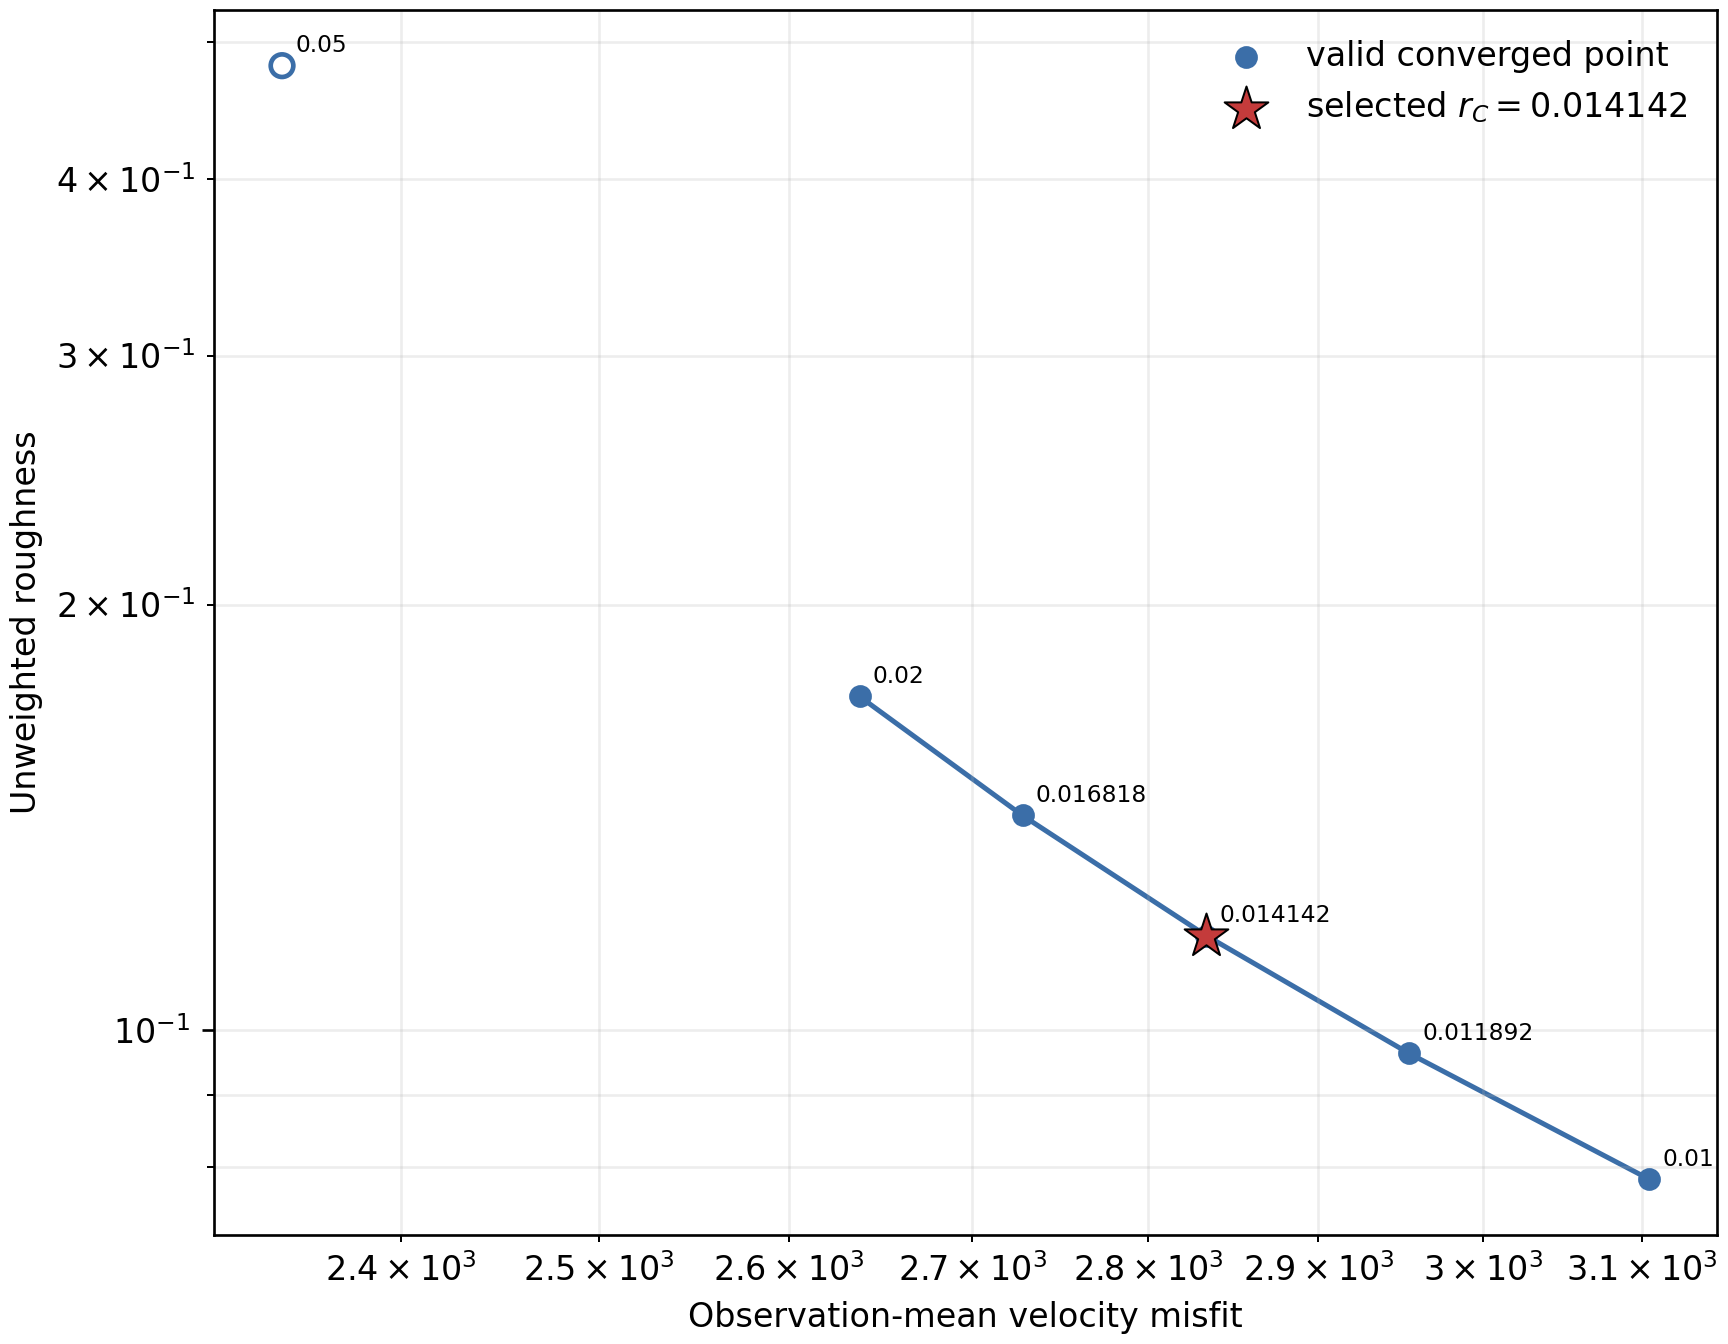
\includegraphics[width=0.82\linewidth]{lcurve_appendix.png}
\caption{L-curve for the sector-wide inversion. The maximum-curvature criterion selects $r_C\simeq0.014$; smaller $r_C$ corresponds to stronger smoothing in the objective function in Eqn~\ref{eq:objective}. The neighboring candidate near $r_C\simeq0.017$ has similar curvature, indicating a narrow elbow range. The open point at $r_C=0.05$ has finite comparable objective values but reached the iteration limit and was not used in the selection.}
\label{fig:lcurve}
\end{figure}

\section{Spatial separation and buffer choice}
\label{app:buffer}

For each 50~km evaluation square, we exclude an additional 40~km buffer
from MLP training and validation on all sides, giving a 130~km excluded
footprint. The buffer is intended to reduce the influence of nearby,
spatially correlated training data on the withheld-square test. We chose the
40~km distance before model fitting using the spatial scale of observed
ice-speed variations.

Using MEaSUREs speed $v$, we formed
\begin{equation}
q(\mathbf{x})=\ln\!\left[1+v(\mathbf{x})/v_0\right],\qquad
v_0=1~\mathrm{m~a^{-1}}.
\end{equation}
The logarithm reduces the influence of the fastest outlets, while the offset
keeps the transformation finite where speed approaches zero. We then removed
the broad sector-scale variation using a normalized Gaussian average with a
50~km standard deviation, leaving local variations in log speed. These local
variations have an estimated $1/e$ correlation length of 22.6~km, and their
correlation falls to 0.108 at a separation of 40~km. Varying the Gaussian
scale from 30 to 100~km gives $1/e$ correlation lengths of
16.1--46.0~km.

An independent estimate from fast-tributary widths gave a 90th-percentile width of approximately 36--38~km across speed thresholds of 100, 250, and 500~m~a$^{-1}$. The 50~km test side therefore spans the coarsest 5~km predictors ten times and exceeds this tributary-width estimate. A 40~km buffer reduces the local log-speed-anomaly correlation to 0.108. Increasing the buffer to 50~km reduces it only to 0.072 while increasing each excluded footprint from 16,900 to 22,500~km$^2$, a 33\% increase. Forty kilometres was therefore selected as a balance between separation from training rows and loss of training and validation data. The buffer separates the test square from nearby training locations at a distance where departures from the broad observed-speed trend have a much weaker spatial correlation than at nearby locations. The sector-wide inversion and non-local membrane-stress response still couple the withheld square to the surrounding ice.

\section{Eligible rows, predictor construction, and support}
\label{app:predictor_population}

This section defines the common set of observation-grid rows used across all
predictor configurations, describes how the derived predictors are constructed,
and explains how predictor support is evaluated in the held-out regions.

We begin by defining the rows eligible for model training and evaluation. The
MEaSUREs velocity raster subset covering the study region contains 2,640,250
pixels. Requiring both observed velocity components to be finite and the
MEaSUREs source flag to be positive retains 2,294,138 paired-velocity pixels;
1,622,598 of these lie inside the computational mesh. All twelve predictors
are finite at those mesh-contained rows. Applying $\phi>0.1$ leaves 1,530,992
common eligible rows, which are used by every predictor configuration. No
additional rows are removed for individual configurations.

For the ten square experiments, excluding the 130~km footprint leaves 1,447,471--1,463,861 rows available for training and validation. Each MLP's reproducible 90/10 split contains 1,302,723--1,317,474 training rows and 144,748--146,387 validation rows. The central-square evaluation sets contain 12,321 rows, except SQ03, which contains 12,432. For each training realization, every predictor configuration uses the same training locations and the same validation locations. Rows outside the common grounded eligible area retain inversion-reference $C$ in every forward simulation. White or uncolored regions in maps denote locations outside the area shown for that experiment or outside that common mask; they were not removed on the basis of target values or model performance.

Surface elevation $s$, thickness $h$, and bed elevation $b$ are represented
as finite-element scalar fields. Their gradients are evaluated as
finite-element vector expressions, interpolated component-wise to the
observation grid, and summarized as
$\lVert\nabla f\rVert=(f_x^2+f_y^2)^{1/2}$ for
$f\in\{s,h,b\}$. Driving-stress magnitude is
\begin{equation}
\tau_d=\rho_i g h\lVert\nabla s\rVert,
\end{equation}
reported in the stress unit used by Icepack, MPa.

The alignment predictor is given by Eqn~\ref{eq:alignment}. The small-gradient
scales were estimated by dividing representative elevation-error scales by the
median mesh-edge length of 6553.4~m. For the surface, a 1~m elevation-error
scale based on the reported REMA accuracy gives
$\epsilon_s=1.5\times10^{-4}$~m~m$^{-1}$. For the bed, the median BedMachine
bed-elevation error over grounded mesh points is 35.31~m, giving
$\epsilon_b=5.4\times10^{-3}$~m~m$^{-1}$. The resulting values were rounded and fixed before model evaluation. The
alignment value is clipped to $[-1,1]$. The $\epsilon_b$ and $\epsilon_s$
terms in the denominator reduce the magnitude of the alignment toward zero
where either gradient is small relative to its corresponding scale.

The selected ice-product and geophysical-product subsets came from an earlier catchment-level comparison of modeled velocity and were specified before the present spatial results were examined. Table~\ref{tab:predictor_provenance} summarizes the native spatial resolution and interpretation of the products used. Interpolation to the observation grid increases the number of sampled values but does not add new spatial information.

\begin{table*}
\caption{Sources and source-grid spacing of the predictors. Nominal cells
in a 50~km square are geometric counts before masks and are not necessarily
independent samples. Derived gradients retain the resolution limits of their
source fields.}
\label{tab:predictor_provenance}
\centering\scriptsize
\setlength{\tabcolsep}{3pt}
\begin{tabular}{>{\raggedright\arraybackslash}p{0.17\textwidth}
                >{\raggedright\arraybackslash}p{0.19\textwidth}
                >{\centering\arraybackslash}p{0.12\textwidth}
                >{\centering\arraybackslash}p{0.10\textwidth}
                >{\raggedright\arraybackslash}p{0.30\textwidth}}
\toprule
Predictor(s) & Product/source & Source grid & Nominal cells & Interpretation in this study\\
\midrule
$s,h,b$ and their gradients & BedMachine Antarctica v2 & 500~m & $\sim$10,000 & Geometry products. Fast-flow bed reconstruction uses mass conservation and velocity, and is not a direct measurement of local basal processes.\\
$\tau_d$ & Derived from BedMachine $h,s$ & 500~m source fields & $\sim$10,000 & Large-scale driving-stress estimate derived from thickness and surface slope.\\
$T_s$ & Quantarctica surface-air-temperature raster & 5~km & $\sim$100 & Large-scale surface thermal boundary, not a direct observation of basal temperature.\\
$Q_b$ & Quantarctica geothermal-heat-flux raster & 5~km & $\sim$100 & Model-derived regional basal heat-flux estimate; interpolation does not add fine-scale information.\\
$m_a$ & ADMAP-2S EPSG:3031 grid & 5~km & $\sim$100 & Magnetic anomaly containing broad information about crustal magnetization; it does not uniquely identify basal material.\\
$g_d$ & AntGG2021 oriented EPSG:3031 grid & 5~km & $\sim$100 & Gravity disturbance containing information about subsurface density; it does not uniquely identify rock type or subglacial water.\\
$a_{bs}$ & Derived from BedMachine $b,s$ & 500~m source fields & $\sim$10,000 & Relative alignment of two geometry gradients; does not use flow direction.\\
\bottomrule
\end{tabular}
\end{table*}

Marginal support is evaluated separately for each predictor. A held-out point
satisfies the marginal criterion when every predictor included in that
configuration lies within the 1st--99th percentile range of the corresponding
eligible non-held-out rows.

Joint support evaluates the full combination of predictor values. Predictor values on a fixed 5~km grid covering the sector are first converted to rank-based normal scores by matching their ranks to standard-normal quantiles \citep{beasley2009rank}. We then use principal component analysis (PCA; \citealp{jolliffe2016principal}) to reduce the predictor space while retaining at least 99\% of the variance of the transformed predictors, and scale the retained components to unit variance. The same transformation is used for all spatial experiments.

To define the joint-support criterion used in square selection and later
evaluation, we use this grid to establish what counts as a sufficiently similar
predictor combination. For each grid point, we calculate the distance in
transformed predictor space to the most similar point located at least 40~km
away geographically. The 95th percentile of these distances defines the
joint-support threshold for that predictor configuration. For each held-out
point, we then find the most similar 5~km reference-grid point within the corresponding training region. The held-out point satisfies the joint criterion when this distance does not exceed the threshold.

Reported predictor support is the area fraction satisfying both the marginal and joint criteria. All held-out points are retained in the modeled velocity evaluation regardless of support.

\section{Basal-friction control: distributions and comparisons}
\label{app:target_distributions}

We first check whether the reference $C$ values in each held-out region fall within the range of values available in the training-and-validation region. This is separate from predictor support, which considers only the input variables. Reference $C$ was not used to select the square locations, define predictor support, or remove evaluation rows.

Figures~\ref{fig:square_target_distributions},~\ref{fig:regional_target_distributions} and Table~\ref{tab:target_distributions} compare the reference $C$ distributions in the training-and-validation and held-out regions. All predictor configurations within a given experiment use the same combined training-and-validation and held-out rows, so the reference-$C$ distributions are also the same for all configurations in that experiment.

\begin{figure*}
\centering
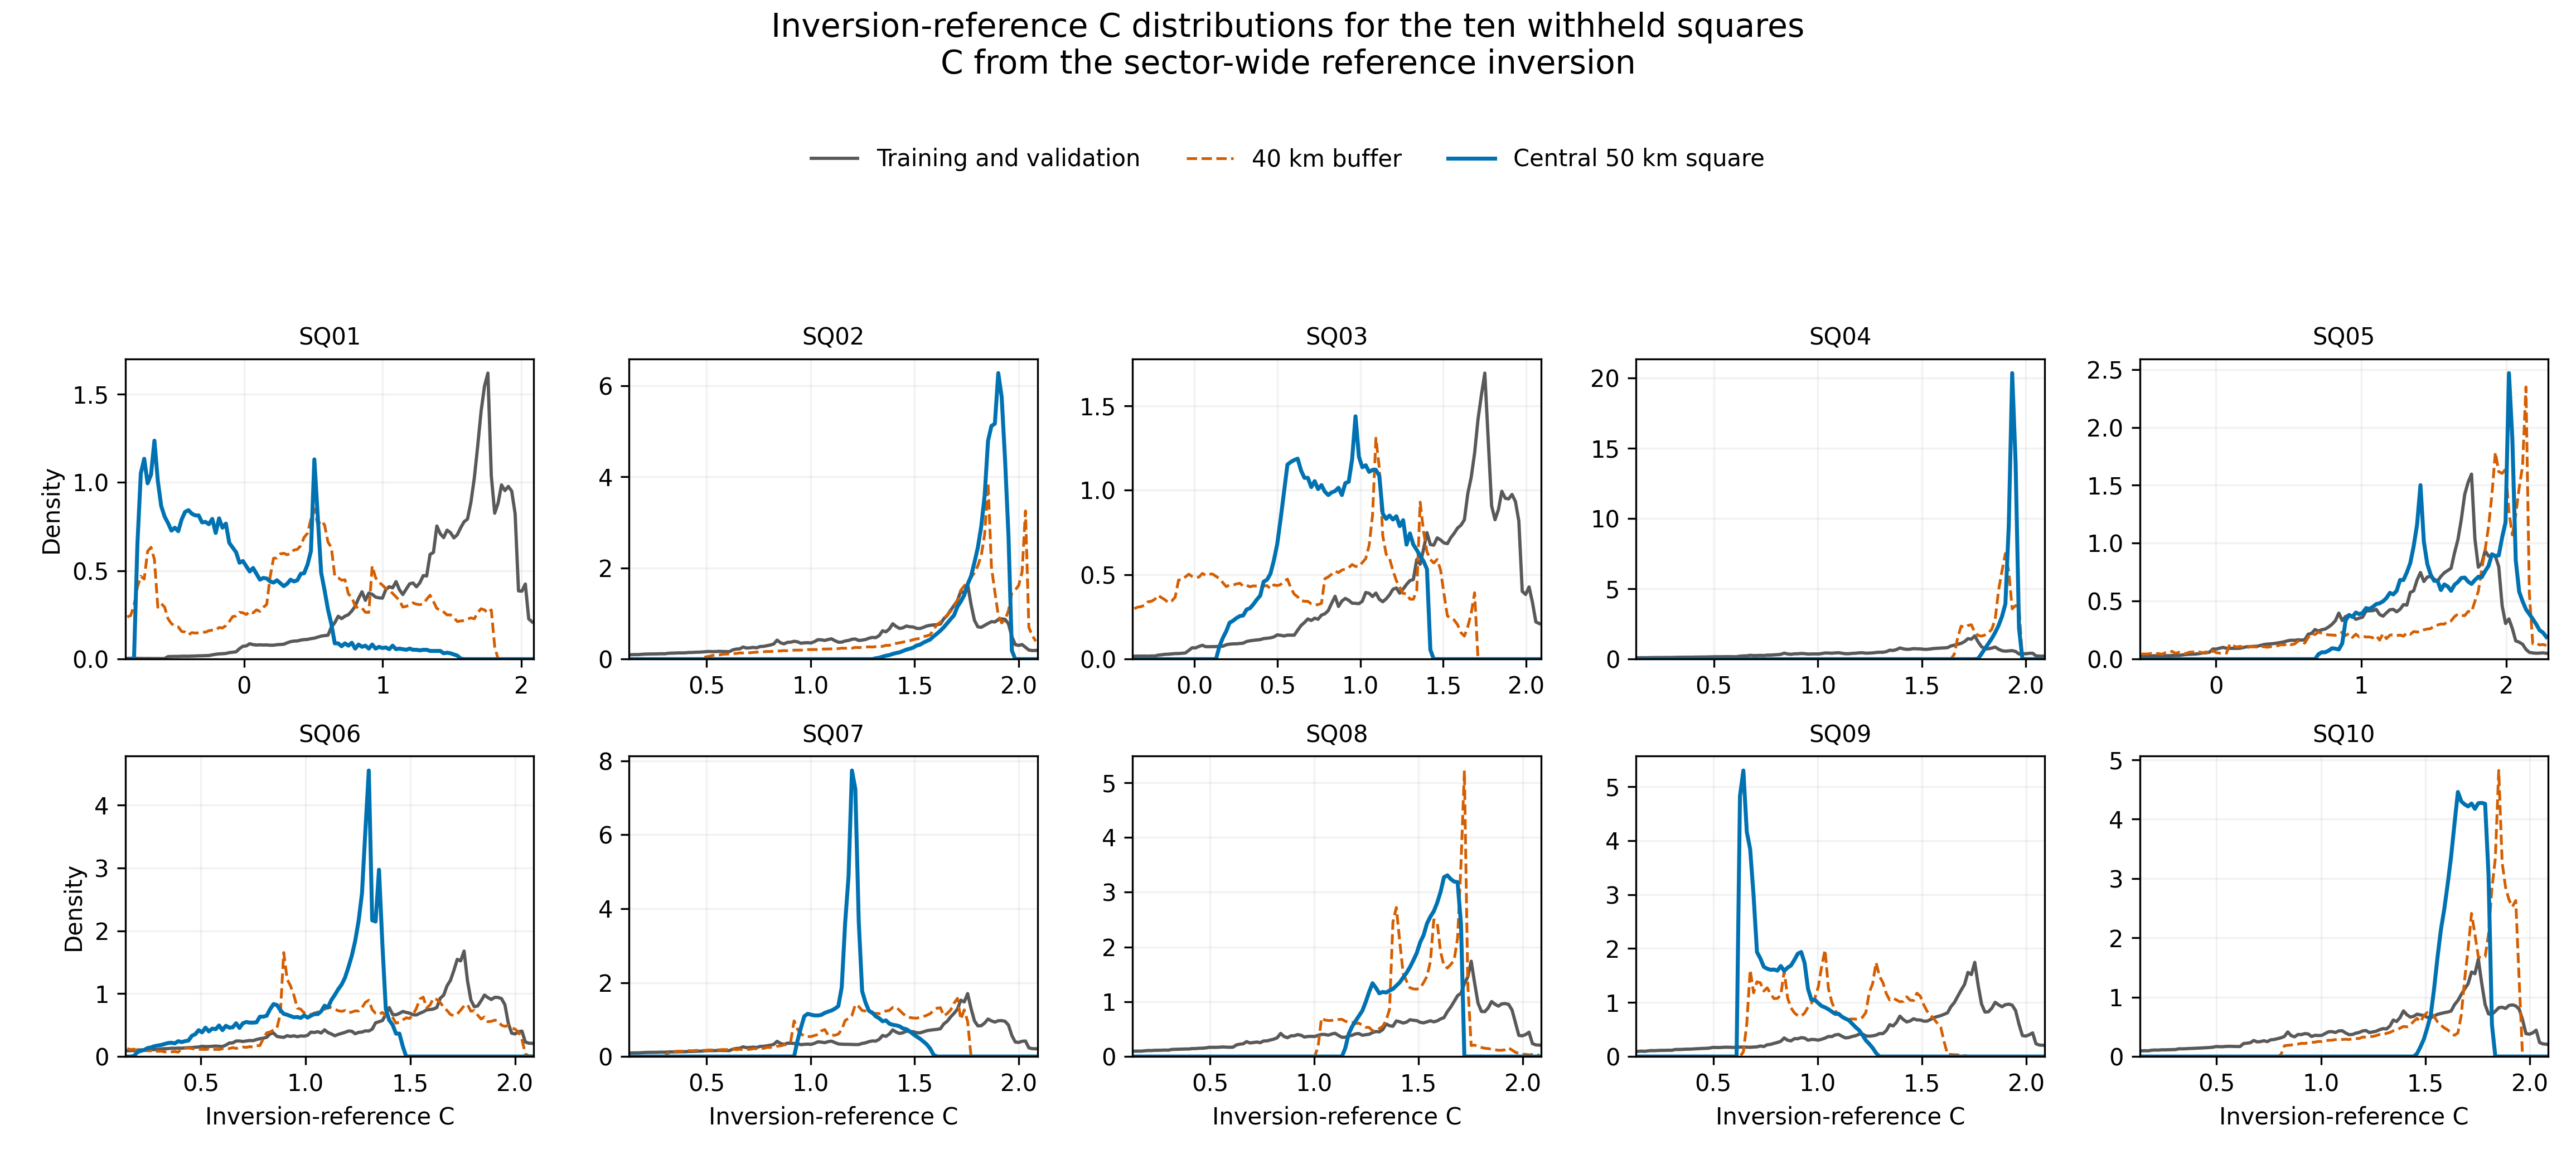
\includegraphics[width=0.99\textwidth]{square_target_distributions.png}
\caption{Reference-$C$ distributions for the ten withheld squares. Each panel
compares the training and validation rows with the central 50~km evaluation
square and the surrounding buffer. The horizontal range is chosen separately
for each panel to show the central part of the distributions clearly. Each
density is normalized using all rows in its set, including values outside the
displayed range. Numerical 1st--99th-percentile intervals and the percentage
of held-out values within the training-and-validation interval are reported in
Table~\ref{tab:target_distributions}. Reference $C$ was not used to select
square locations or remove evaluation rows.}
\label{fig:square_target_distributions}
\end{figure*}

\begin{figure*}
\centering
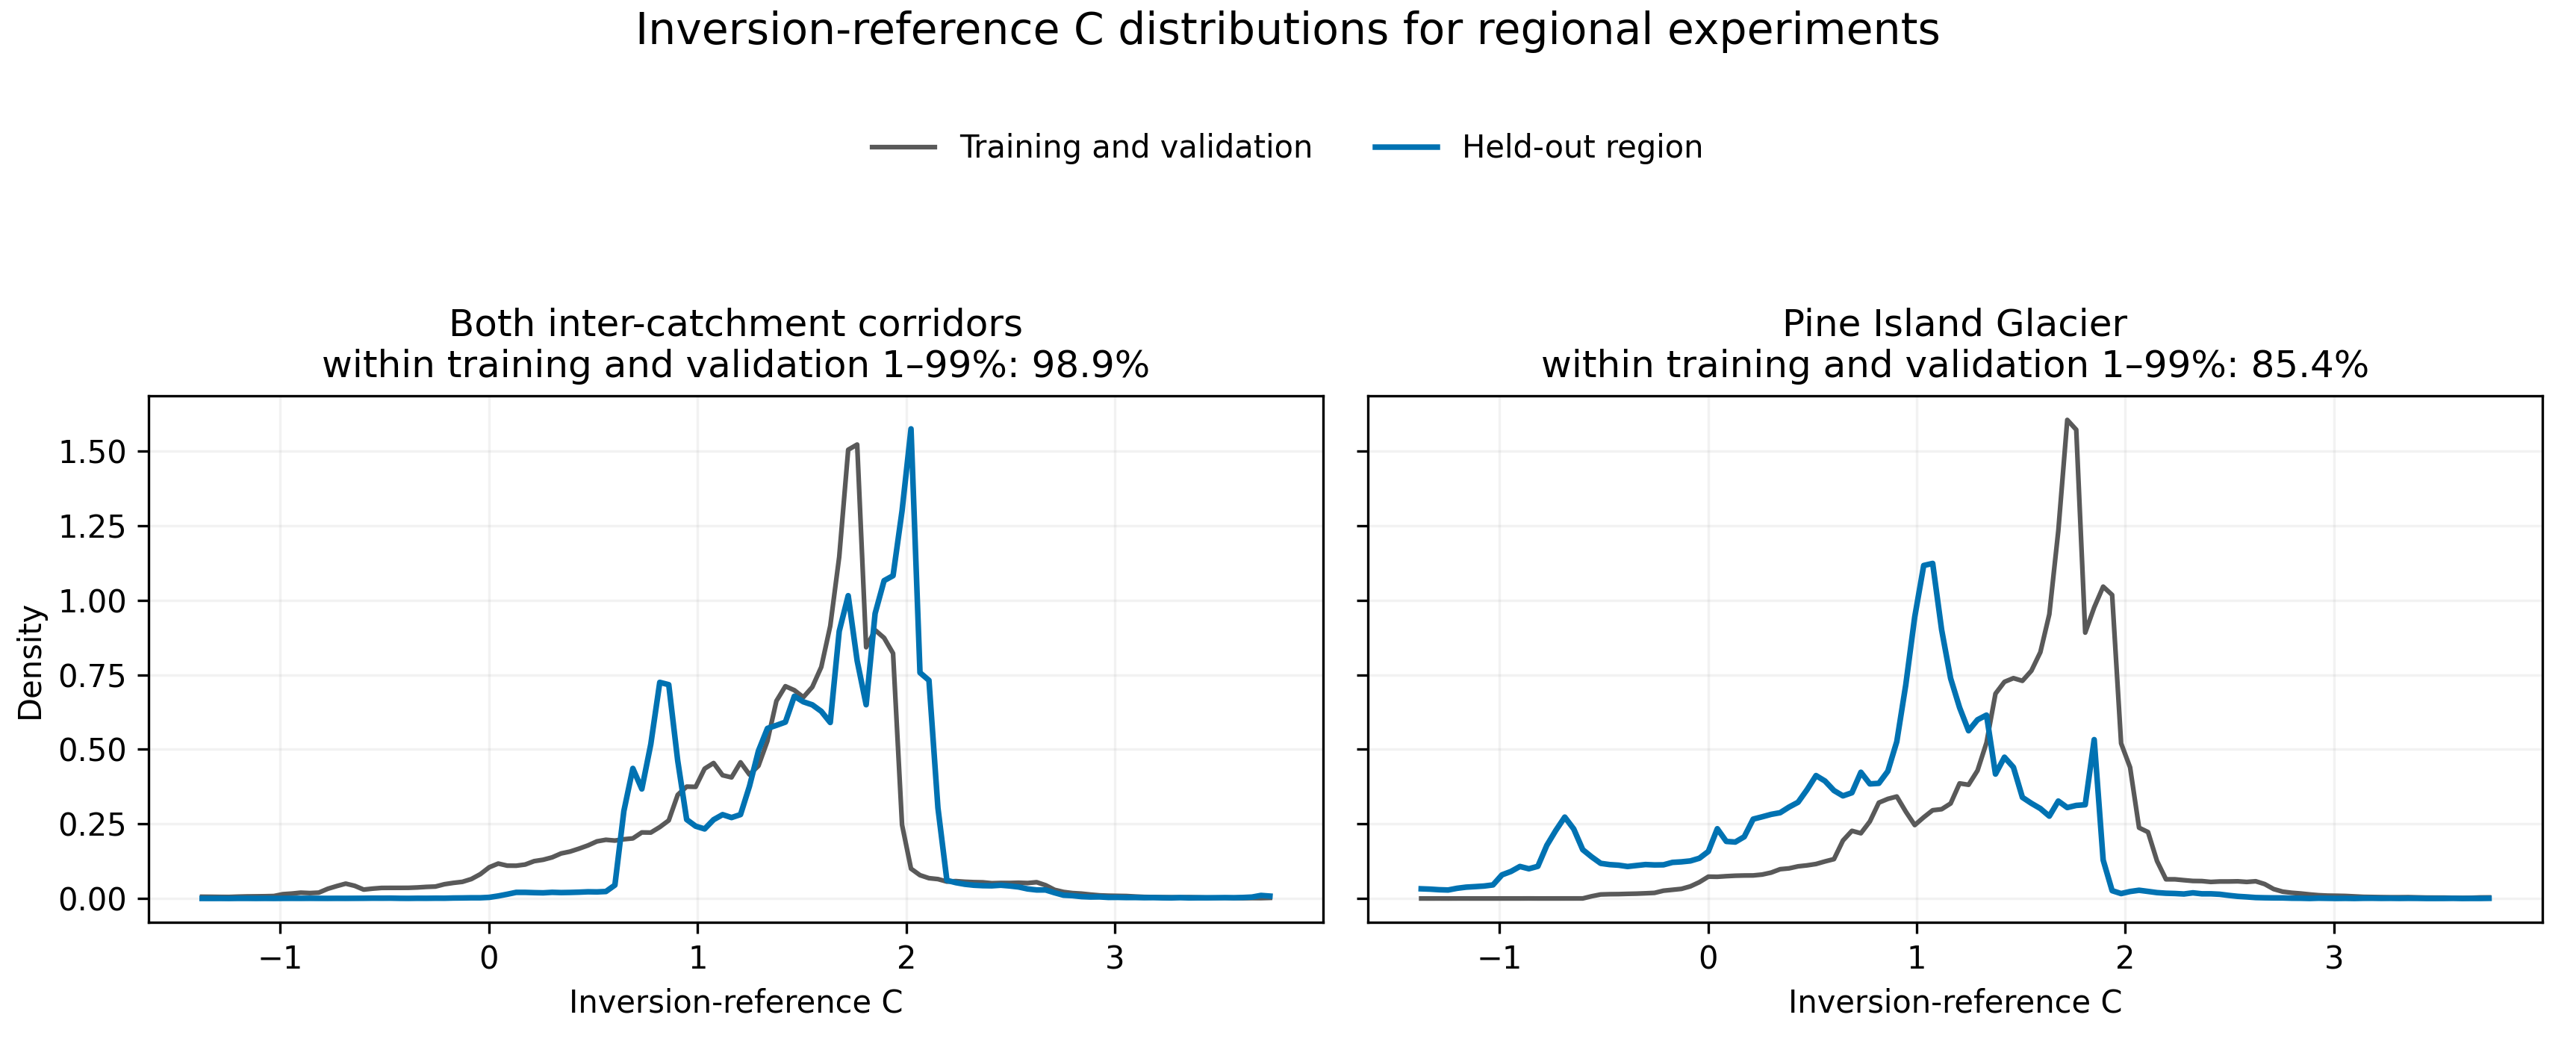
\includegraphics[width=0.92\textwidth]{regional_target_distributions.png}
\caption{Reference-$C$ distributions for the two regional tests. Each panel
compares the training and validation rows with the complete held-out region.
The percentage shown is the fraction of held-out $C$ values that falls within
the 1st--99th-percentile range of the training and validation data.}
\label{fig:regional_target_distributions}
\end{figure*}

\begin{table*}
\caption{Reference-$C$ distributions in the training-and-validation and held-out regions. Intervals are the 1st--99th percentiles of dimensionless $C$. The final column gives the percentage of held-out rows whose $C$ values fall within the corresponding training-and-validation interval.}
\label{tab:target_distributions}
\centering\scriptsize
\setlength{\tabcolsep}{3pt}
\begin{tabular}{lrrrrr}
\toprule
Experiment & \shortstack{Training and\\validation rows} & Held-out rows &
\shortstack{Training and\\validation interval} & Held-out interval &
\shortstack{Held-out within\\training range (\%)}\\
\midrule
SQ01 & 1,448,295 & 12,321 & $-0.22$--$2.67$ & $-0.76$--$1.30$ & 51.9\\
SQ02 & 1,447,471 & 12,321 & $-0.69$--$2.67$ & $1.43$--$1.96$ & 100.0\\
SQ03 & 1,450,403 & 12,432 & $-0.69$--$2.67$ & $0.21$--$1.40$ & 100.0\\
SQ04 & 1,447,471 & 12,321 & $-0.69$--$2.67$ & $1.80$--$1.96$ & 100.0\\
SQ05 & 1,459,429 & 12,321 & $-0.65$--$2.66$ & $0.84$--$2.35$ & 100.0\\
SQ06 & 1,447,471 & 12,321 & $-0.69$--$2.67$ & $0.28$--$1.43$ & 100.0\\
SQ07 & 1,447,471 & 12,321 & $-0.69$--$2.67$ & $0.95$--$1.55$ & 100.0\\
SQ08 & 1,453,825 & 12,321 & $-0.69$--$2.66$ & $1.18$--$1.71$ & 100.0\\
SQ09 & 1,458,393 & 12,321 & $-0.69$--$2.66$ & $0.62$--$1.23$ & 100.0\\
SQ10 & 1,463,861 & 12,321 & $-0.69$--$2.66$ & $1.50$--$1.81$ & 100.0\\
Inter-catchment & 1,241,683 & 289,309 & $-0.72$--$2.65$ & $0.49$--$2.66$ & 98.9\\
PIG & 1,303,307 & 227,685 & $-0.08$--$2.69$ & $-1.28$--$2.05$ & 85.4\\
\bottomrule
\end{tabular}
\end{table*}

These comparisons show how the reference-$C$ range in each held-out region overlaps that in the training-and-validation region; modeled velocity tests whether the predicted control reproduces the observed flow. The reference $C$ is one regularized, model-dependent inversion solution, and modeled velocity remains the primary evaluation in this study.

We measure agreement with the inversion-reference control using $C$ RMSE and the coefficient of determination $R_C^2$. The latter is one minus the sum of squared prediction errors divided by the sum of squared deviations of reference $C$ from its mean over the same evaluated locations.

Table~\ref{tab:validation_c_diagnostics} reports agreement with the inversion-reference control on the validation rows. Each MLP was evaluated on its own validation rows, so the table reports the median of the ten member-level results for each square--configuration experiment. Validation $C$ RMSE is lower and $R_C^2$ higher for the other five configurations than for CFG04. The contrast with the spatially held-out results in Table~\ref{tab:c_diagnostics} shows that agreement on randomly withheld rows within the training region does not imply comparable transfer to a spatially separated square.

\begin{table*}
\caption{Validation agreement with the inversion-reference control. Each
entry is the median $C$ RMSE / $R_C^2$ across the ten MLP members for that
square--configuration experiment, calculated on each member's own validation
rows. RMSE is in the dimensionless control $C$, and $R_C^2$ is dimensionless.
The validation rows lie outside the excluded 130~km footprint and were used for selection of the fitted MLP; they are not independent test data.}
\label{tab:validation_c_diagnostics}
\centering
\scriptsize
\setlength{\tabcolsep}{4pt}
\begin{tabular}{lrrrrrr}
\toprule
Square & CFG01 & CFG02 & CFG03 & CFG04 & CFG05 & CFG06\\
\midrule
SQ01 & 0.077/0.984 & 0.075/0.985 & 0.056/0.992 & 0.363/0.652 & 0.020/0.999 & 0.022/0.999 \\
SQ02 & 0.078/0.987 & 0.081/0.986 & 0.057/0.993 & 0.387/0.680 & 0.023/0.999 & 0.022/0.999 \\
SQ03 & 0.072/0.988 & 0.077/0.986 & 0.070/0.989 & 0.383/0.661 & 0.022/0.999 & 0.021/0.999 \\
SQ04 & 0.080/0.986 & 0.079/0.986 & 0.056/0.993 & 0.393/0.666 & 0.023/0.999 & 0.022/0.999 \\
SQ05 & 0.076/0.987 & 0.077/0.986 & 0.055/0.993 & 0.364/0.697 & 0.023/0.999 & 0.021/0.999 \\
SQ06 & 0.073/0.988 & 0.080/0.986 & 0.057/0.993 & 0.382/0.681 & 0.022/0.999 & 0.022/0.999 \\
SQ07 & 0.077/0.987 & 0.077/0.987 & 0.058/0.993 & 0.388/0.681 & 0.021/0.999 & 0.022/0.999 \\
SQ08 & 0.077/0.988 & 0.079/0.987 & 0.056/0.993 & 0.397/0.669 & 0.022/0.999 & 0.023/0.999 \\
SQ09 & 0.077/0.987 & 0.079/0.986 & 0.057/0.993 & 0.384/0.676 & 0.022/0.999 & 0.022/0.999 \\
SQ10 & 0.077/0.987 & 0.080/0.986 & 0.058/0.993 & 0.391/0.676 & 0.023/0.999 & 0.022/0.999 \\
\bottomrule
\end{tabular}
\end{table*}

We also compare the predicted $C$ fields directly with the reference $C$ to
measure how closely the MLP reproduces the inversion result.
Table~\ref{tab:c_diagnostics} reports $C$ RMSE and $R_C^2$ for every central
square. Negative $R_C^2$ values are retained; a negative value means that the
predicted $C$ has larger squared error than using the mean reference $C$ within
that square. The median $R_C^2$ values across the ten squares are $-1.39$,
$-1.35$, $-7.97$, $-6.52$, $-1.41$, and $-1.21$ for CFG01--CFG06,
respectively. Poor agreement with the reference $C$ can still coexist with improved modeled velocity, so these statistics answer a different question from the velocity comparison.

\begin{table*}
\caption{Comparison between predicted and reference $C$ in the ten central
squares. Each entry gives $C$ RMSE / $R_C^2$ for the median predicted $C$
field. RMSE is in dimensionless $C$ units.}
\label{tab:c_diagnostics}
\centering\scriptsize
\setlength{\tabcolsep}{4pt}
\begin{tabular}{lrrrrrr}
\toprule
Square & CFG01 & CFG02 & CFG03 & CFG04 & CFG05 & CFG06\\
\midrule
SQ01 & 0.42/0.25 & 0.41/0.29 & 1.44/$-8.00$ & 1.21/$-5.42$ & 0.58/$-0.47$ & 0.52/$-0.20$ \\
SQ02 & 0.22/$-2.69$ & 0.22/$-2.46$ & 0.88/$-56.51$ & 0.61/$-26.00$ & 0.17/$-1.04$ & 0.15/$-0.69$ \\
SQ03 & 0.38/$-0.63$ & 0.37/$-0.61$ & 0.54/$-2.31$ & 0.54/$-2.32$ & 0.35/$-0.38$ & 0.33/$-0.29$ \\
SQ04 & 0.20/$-29.81$ & 0.20/$-30.02$ & 0.36/$-98.61$ & 0.33/$-80.67$ & 0.16/$-18.76$ & 0.16/$-18.71$ \\
SQ05 & 0.37/0.03 & 0.37/0.02 & 0.46/$-0.50$ & 0.48/$-0.63$ & 0.41/$-0.21$ & 0.42/$-0.25$ \\
SQ06 & 0.52/$-1.83$ & 0.51/$-1.72$ & 0.51/$-1.77$ & 0.47/$-1.35$ & 0.33/$-0.14$ & 0.34/$-0.19$ \\
SQ07 & 0.24/$-2.44$ & 0.23/$-2.18$ & 0.57/$-17.72$ & 0.52/$-14.99$ & 0.30/$-4.13$ & 0.31/$-4.77$ \\
SQ08 & 0.20/$-0.96$ & 0.20/$-0.98$ & 0.28/$-2.78$ & 0.31/$-3.43$ & 0.24/$-1.77$ & 0.24/$-1.73$ \\
SQ09 & 0.74/$-18.37$ & 0.74/$-18.49$ & 0.87/$-26.27$ & 0.49/$-7.63$ & 0.53/$-8.90$ & 0.51/$-8.38$ \\
SQ10 & 0.10/$-0.79$ & 0.10/$-0.83$ & 0.23/$-7.93$ & 0.31/$-14.95$ & 0.31/$-15.21$ & 0.27/$-11.59$ \\
\bottomrule
\end{tabular}
\end{table*}


For the PIG holdout experiment, the median validation $C$ RMSE /
$R_C^2$ across the ten MLP members is 0.081/0.981 for CFG01,
0.077/0.983 for CFG02, and 0.056/0.991 for CFG03. These values
were calculated on each member's own validation rows outside the
withheld PIG region. Despite this strong validation agreement, the
corresponding median predicted fields have PIG holdout $C$ RMSE /
$R_C^2$ values of 0.92/$-0.49$, 0.85/$-0.28$, and
1.23/$-1.69$, respectively. Thus, performance on randomly withheld
validation rows does not predict spatial transfer to the withheld
catchment. 

The inter-catchment experiment provides an additional regional test by withholding the complete PIG--Thwaites and Thwaites--Dotson corridors. This tests transfer from the named glacier catchments to the regions between them. For the two corridors together, the holdout $C$ RMSE / $R_C^2$ values are 0.81/$-1.86$, 0.33/0.53, and 0.33/0.52 for CFG04--CFG06. Across both corridors, the median predicted $C$ fields give velocity RMSE values of 470.3, 119.0, and 109.3~m~a$^{-1}$ for CFG04, CFG05, and CFG06, respectively, compared with 578.4~m~a$^{-1}$ for uniform $C$ and 28.1~m~a$^{-1}$ for the inversion reference. The corresponding relative RMSE values are 0.81, 0.21, and 0.19. The two corridors are spatially separate, and the intervening region is not included in the calculation. All three configurations reduce velocity RMSE relative to uniform $C$ over the combined corridor area, with lower errors for CFG05 and CFG06 than for CFG04.
For these velocity calculations, all four controls replace the inversion
reference only inside the combined corridor geography and retain the same
reference $C$ outside it, matching the controlled comparison used for the
square and PIG CFG02 results.

Finally, we examine the small number of unusually large reference-$C$ values
because mean-square loss gives large prediction residuals greater weight.
Across all eligible rows, $C$ has a median of 1.54, a
1st--99th-percentile range of $-0.68$ to 2.65, a 99.9th percentile of
3.76, and a maximum of 24.18. Values greater than 5 occur in only 821 of
1,530,992 rows (0.054\%). They are more common near the grounding
transition but are not confined to it: 261 occur where
$0.1<\phi\leq0.2$. The scaling used for training changes the numerical
scale of $C$ but does not selectively reduce the contribution of large
prediction residuals. The largest 0.1\% of squared deviations from the
target median account for 12.5\% of the total squared deviation.

For the MLPs selected by minimum validation MSE, rows with $C>5$ account for a median of 1.59\% of validation squared error; excluding them from validation scoring reduces median validation RMSE by 0.77\% and does not materially alter the configuration comparisons. No such rows occur in the ten central squares or the PIG evaluation region, so we retain them rather than introduce a target-based exclusion and retraining step. These rare large values are features of the inversion-derived target and should not be interpreted as direct evidence for extreme physical basal resistance.

\subsection{Training representation and prediction error}
\label{app:training_representation}

We also test whether prediction errors are related to how densely the predictor values at each held-out location are represented in the training data. For CFG02 and CFG04 in the ten central 50~km squares, and CFG02 in PIG, we calculate $d_{20}$ for each held-out row, defined as the distance to its 20th-nearest training row. Nearest-neighbor distances underlie multivariate density estimation \citep{loftsgaarden1965nonparametric}; here $d_{20}$ describes training representation rather than estimating a probability density. Distances are calculated after applying the same transformation used for joint support: predictor ranks are mapped to normal scores, followed by PCA retaining at least 99\% of the variance, with the retained components scaled to unit variance. This transformation is fitted to the eligible sector-wide 5~km grid. Smaller $d_{20}$ values indicate that many similar predictor combinations occur in the training data, whereas larger values indicate sparser representation. Unlike the joint-support calculation, no minimum geographic separation is imposed here; all training rows are used, including nearby rows and repeated predictor combinations.

For each MLP realization, 10,000 training rows are sampled uniformly without
replacement. The $d_{20}$ value for each sampled training row is calculated
against the complete training set, excluding only that row itself. These
10,000 values provide a reference distribution for the held-out rows. Each
held-out $d_{20}$ value is assigned the percentile

\begin{equation}
p=100\frac{N(d_{20,\mathrm{train}}<d_{20,\mathrm{test}})
+\tfrac{1}{2}N(d_{20,\mathrm{train}}=d_{20,\mathrm{test}})}
{10{,}000}.
\end{equation}

For each held-out row, we use the median percentile across the ten MLP realizations for that experiment and configuration. Higher percentiles indicate sparser representation in the training data. We group the held-out rows into three categories: $p\leq50$, $50<p\leq95$, and $p>95$. The neighbor count and category boundaries were fixed before examining prediction errors.

We examine the original training data without rebalancing. The predictors are continuous and several are physically or mathematically related. Balancing each predictor separately would not necessarily balance combinations of predictors and could change the relative frequency of the combinations present in the original data. Instead, this analysis measures how densely the existing training data represent each held-out predictor combination.

To compare training representation with prediction error, the median predicted $C$ field is evaluated on the same 450~m observation-grid rows used for the representation analysis. The median is first calculated on the model mesh and then interpolated to the observation grid in the same way as the reference $C$. All central-square rows are retained. The PIG analysis uses the same procedure over its complete eligible held-out area. Within each representation category, we calculate $C$ RMSE, mean signed difference, and mean absolute difference from the reference $C$. Velocity RMSE and relative RMSE are calculated over the same rows.

The whole-square $C$ RMSE values calculated on the regular 450~m grid differ by
at most 2.37\% from the area-weighted values in
Table~\ref{tab:c_diagnostics}, which are calculated on the finite-element
mesh. All $C$ errors are reported in the original dimensionless $C$ units.

\begin{table*}
\centering\small
\caption{Prediction error in $C$ relative to the inversion reference and training representation in the central squares. The three columns give dimensionless $C$ RMSE for increasingly sparse representation categories. Spearman $\rho$ relates the representation percentile of each row to its absolute $C$ error within each square. The last row for each configuration gives the median across the ten squares.}
\label{tab:representation_c}
\begin{tabular}{llrrrr}
\toprule
Configuration & Square & $p\leq50$ & $50<p\leq95$ & $p>95$ & $\rho$\\
\midrule
CFG02 & SQ01 & 0.371 & 0.410 & 0.418 & 0.076\\
 & SQ02 & 0.206 & 0.232 & 0.265 & 0.107\\
 & SQ03 & 0.370 & 0.384 & 0.411 & 0.086\\
 & SQ04 & 0.201 & 0.204 & 0.211 & 0.056\\
 & SQ05 & 0.416 & 0.351 & 0.337 & $-0.141$\\
 & SQ06 & 0.493 & 0.516 & 0.543 & 0.035\\
 & SQ07 & 0.227 & 0.242 & 0.245 & 0.090\\
 & SQ08 & 0.175 & 0.212 & 0.198 & 0.133\\
 & SQ09 & 0.731 & 0.735 & 0.753 & 0.062\\
 & SQ10 & 0.130 & 0.103 & 0.110 & $-0.087$\\
 & Median & 0.299 & 0.297 & 0.301 & 0.069\\
\midrule
CFG04 & SQ01 & 1.100 & 1.298 & 1.058 & $-0.101$\\
 & SQ02 & 0.608 & 0.634 & 0.470 & $-0.049$\\
 & SQ03 & 0.512 & 0.572 & 0.587 & 0.139\\
 & SQ04 & 0.375 & 0.364 & 0.236 & $-0.637$\\
 & SQ05 & 0.473 & 0.508 & 0.422 & 0.065\\
 & SQ06 & 0.383 & 0.515 & 0.474 & 0.224\\
 & SQ07 & 0.634 & 0.477 & 0.466 & $-0.257$\\
 & SQ08 & 0.348 & 0.307 & 0.309 & $-0.044$\\
 & SQ09 & 0.517 & 0.491 & 0.411 & $-0.055$\\
 & SQ10 & 0.299 & 0.317 & 0.302 & $-0.094$\\
 & Median & 0.492 & 0.499 & 0.444 & $-0.052$\\
\bottomrule
\end{tabular}
\end{table*}

Table~\ref{tab:representation_c} tests whether $C$ prediction error increases
as training representation becomes sparser. For CFG02, $C$ RMSE increases
from the better-represented to the more sparsely represented categories in
seven of the ten squares. However, this pattern is not consistent across the
full set of experiments. The median $C$ RMSE across the ten squares is 0.299,
0.297, and 0.301 for $p\leq50$, $50<p\leq95$, and $p>95$, respectively, and
the median within-square Spearman correlation between representation
percentile and absolute $C$ error is only 0.069. Thus, although some individual
squares show larger $C$ errors where similar training examples are sparser,
training representation does not provide a general explanation for $C$
prediction error. CFG04 shows even less evidence of such a relationship:
only one square has increasing $C$ RMSE across the three categories, and the
median within-square correlation is $-0.052$.

To test whether the weak relationship between training representation and
$C$ error is being obscured by differences in ice speed, we repeat the
analysis within observed-speed classes. For each class, the correlation is
between representation percentile and absolute $C$ error. Below
100~m~a$^{-1}$, the median within-square correlations are 0.080 for CFG02
and $-0.113$ for CFG04. Between 100 and 500~m~a$^{-1}$, they are 0.079 and
0.015, respectively. These values remain close to zero, indicating that
sparser training representation is not consistently associated with larger
$C$ error within either the slow- or moderate-flow classes. Only one square
contributes to the 500--1000~m~a$^{-1}$ class, so there are not enough
repeated spatial tests to draw the same conclusion for faster flow.

Relative velocity RMSE also does not vary consistently with training representation. In SQ06, CFG02 performs worse than uniform $C$ in the best-represented category (relative velocity RMSE 1.15) but improves on uniform $C$ in the sparsest category (0.96). In SQ05, $C$ RMSE decreases from 0.416 to 0.337 between these categories (Table~\ref{tab:representation_c}), while relative velocity RMSE increases from 0.37 to 0.81. In SQ02--CFG04, the best-represented category has a $C$ RMSE of 0.608 and a relative velocity RMSE of 1.45, whereas the sparsest category has lower $C$ RMSE (0.470) and relative velocity RMSE (1.34). These examples show that sparser training representation does not consistently correspond to larger relative velocity RMSE. They also show that closer agreement with the reference $C$ does not necessarily produce lower relative velocity RMSE.

\section{MLP training and statistical comparisons}
\label{app:training_campaign}

This section describes the MLP architecture and training procedure, the
repeated training realizations used for each experiment, and the statistical
comparisons used to summarize differences among configurations.

The MLP has ten hidden layers of 200 units. Each hidden layer is followed by batch normalization and a SiLU activation, and the final layer is linear. Predictors and $C$ are robustly scaled using medians and interquartile ranges fitted on training rows only. Adam uses an initial learning rate of $10^{-3}$ and batch size 1024, with reproducible epoch-wise shuffling. The learning rate is multiplied by 0.2, down to $10^{-6}$, after 15 epochs without a validation-MSE decrease of at least $10^{-4}$. Training stops after 45 epochs without improvement in validation MSE, and the fitted MLP with the lowest unpenalized validation MSE is used.

A separate CFG06 calculation selected the L2 penalty without using any of the ten central squares. Its fixed 70/20/10 split contained 1,407,671 rows: 985,369 for training, 281,534 for validation, and 140,768 for testing. L2 penalties of 0, $10^{-6}$, $10^{-5}$, and $10^{-4}$ were applied to the hidden-layer weights and compared using unpenalized validation MSE. The respective minimum values were 0.001207, 0.001332, 0.001583, and 0.003117. No nonzero penalty reduced validation MSE below that of the zero-penalty model, so all final MLP trainings used $\lambda_{\mathrm{L2}}=0$. The test rows were not used to choose the penalty. 

We did not optimize the network architecture separately for each predictor
configuration or held-out region. Instead, we used the same relatively large
network, with ten hidden layers of 200 units, for all experiments. This
architecture provides substantial flexibility to represent nonlinear
relationships between the predictors and $C$, while keeping the network
design fixed across configurations and spatial tests. Overfitting is limited
through a separate validation set, learning-rate reduction, early stopping,
and restoration of the model with the lowest validation MSE. The training and
validation histories shown below provide an additional check, with no
systematic separation between them during training. A full architecture search
would require separate tuning across multiple predictor configurations and
spatial splits and was beyond the scope of this study. The chosen architecture
should therefore be viewed as a fixed, flexible modeling choice rather than an
optimized architecture.

Each experiment--configuration pair uses ten reproducible training realizations with different training/validation row assignments, initial weights, and epoch shuffles. We trained 660 MLPs in total. The regional tests use CFG01--CFG03 for PIG and CFG04--CFG06 for the inter-catchment corridors. For each experiment--configuration pair, the ten predicted $C$ fields are combined by taking the median at each mesh vertex, giving 66 median fields. The controlled forward evaluation in the main text uses the 60 square fields and the PIG CFG02 field. The individual realizations are used to assess sensitivity to the training procedure and to construct the median prediction; they are not treated as independent spatial tests or as estimates of predictive uncertainty.

For the velocity-error calculations, modeled velocity is interpolated to the
pixel centres of the regular 450~m MEaSUREs observation grid and compared
with the original paired raster components there. Squared vector residuals are averaged
over the retained grid points before taking the square root. Because the
observation grid has uniform spacing, this provides an equal-area approximation
to the spatial mean rather than an exact finite-element integration.

For the spatially uniform-$C$ reference, the mean inversion-reference $C$ is
calculated from finite-element cells in the non-held-out region. Cell means of
$C$ are weighted by cell area. Geographic membership and the criterion
$\phi>0.1$ are evaluated at cell centers, with positive thickness and finite
$C$ also required. The resulting value therefore uses model cells rather than
observation-grid row means. It is applied over the same withheld footprint or
catchment used for the predicted $C$ field, with inversion-reference $C$
retained elsewhere.

The ten squares are treated as the independent spatial units for statistical comparison. The PIG and inter-catchment experiments are secondary regional tests and do not add independent units to these comparisons. The spatially uniform-$C$ simulation tests whether predictor-dependent spatial variation reduces velocity RMSE relative to uniform $C$; it is not a comparison with another learning algorithm. Results are reported for every square and summarized using the median and interquartile range across the ten squares. Exact paired sign tests compare predictor configurations chosen in advance. The individual MLP realizations, and the central square and full footprint from the same experiment, are not counted as additional independent units. All 66 median predicted $C$ fields are finite. Predictions were not clipped to the range of the inversion-reference $C$.

The complete histories in Fig.~\ref{fig:training_convergence} show that the training and validation losses decrease and then approach a plateau. Median validation MSE decreases from its initial value by factors of 19.5, 19.4, 37.7, 1.68, 148, and 162 for CFG01--CFG06, respectively. Training and validation histories remain close throughout training, with no systematic growth in the gap between them. This provides no clear evidence that the relatively large network is increasingly fitting the training rows at the expense of the validation rows. Validation agreement with the reference $C$ is high for CFG01, CFG02, CFG03, CFG05, and CFG06, while CFG04 shows a much smaller reduction in validation loss and higher validation $C$ RMSE and lower $R_C^2$. However, CFG04 still reduces velocity RMSE relative to uniform $C$ in seven of the ten spatially withheld squares. The main implication is that successful fitting of $C$ on random validation rows within the training region does not by itself predict performance in a spatially separated region. The common architecture and training procedure provide a controlled comparison among predictor configurations, while the spatially withheld tests assess whether the learned relationships produce useful modeled velocities elsewhere.

We used paired sign tests to assess whether one configuration consistently had lower velocity RMSE than another across the ten withheld squares \citep[Chapter~3, Section~3.4]{hollander2013nonparametric}. All 15 possible
pairwise configuration comparisons were tested; none was statistically
significant after Holm correction for multiple comparisons
\citep{holm1979simple}. All 15 Holm-adjusted $p$-values are 1.0. For the five comparisons corresponding directly to
predictor additions or removals in the configuration design, the unadjusted
two-sided $p$-values were 1.0 for CFG02--CFG01, 1.0 for CFG04--CFG03,
0.344 for CFG05--CFG02, 0.344 for CFG05--CFG04, and 1.0 for
CFG06--CFG05. Thus, although some configurations have lower median RMSE or
perform better in more squares, no configuration shows a statistically
significant consistent advantage over another across the ten spatial tests.

\begin{figure*}
\centering
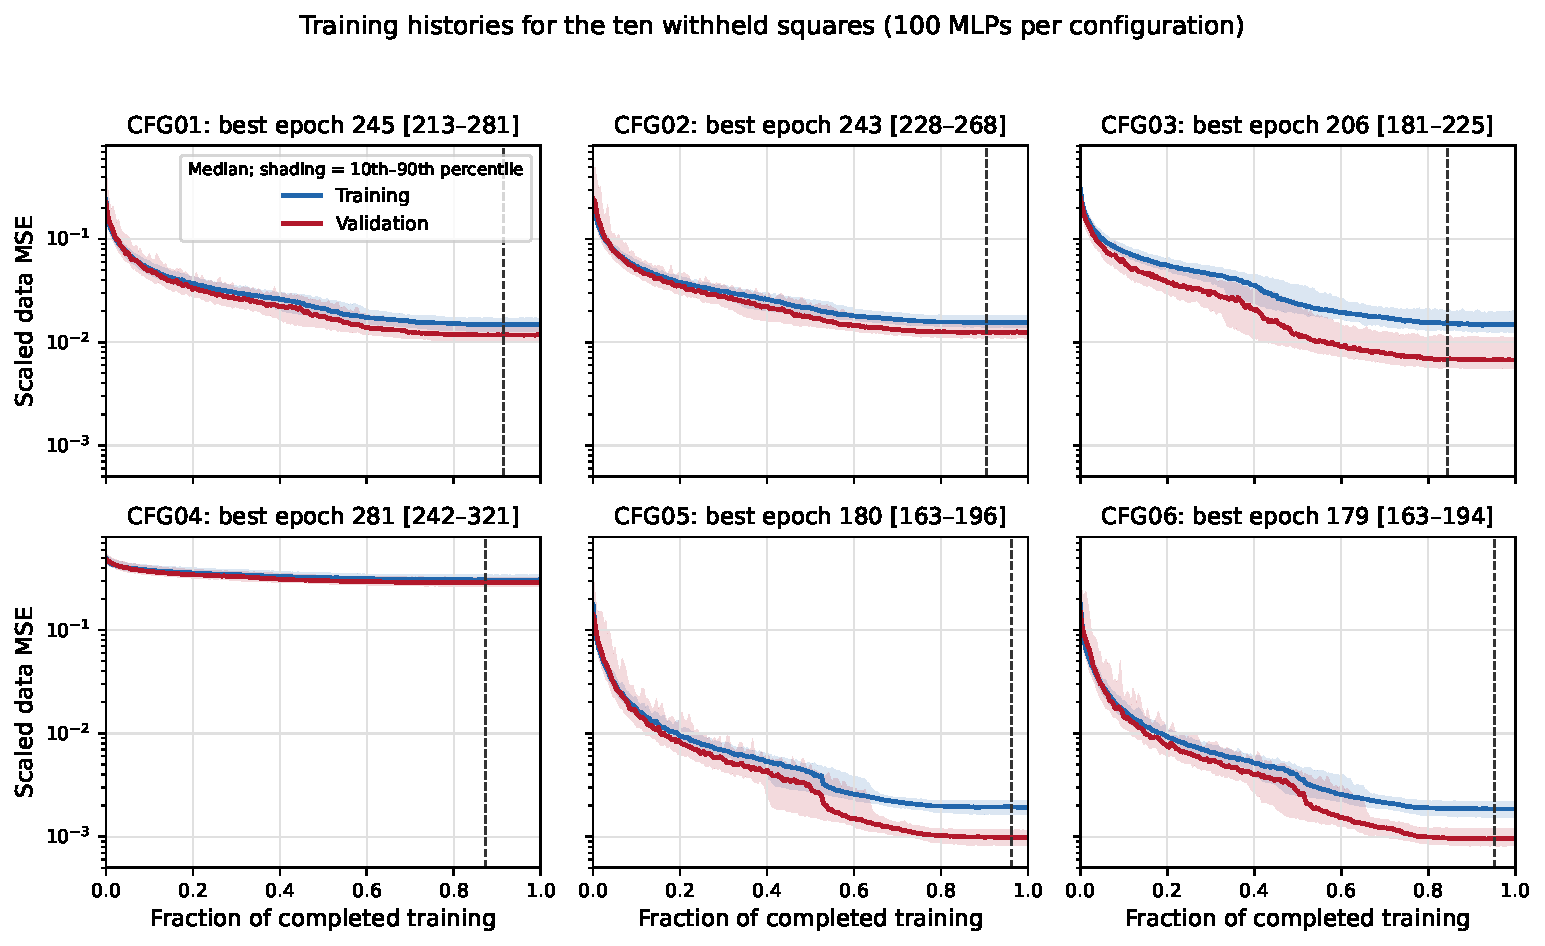
\includegraphics[width=0.98\textwidth]{appendix_training_convergence.pdf}
\caption{Training histories for all 600 primary-square MLP runs, comprising ten squares and ten MLPs for each configuration. To retain every run in the summary, each history is scaled from its first epoch (training fraction zero) to the end of training (training fraction one). Lines show median training and validation data MSE, and shading spans the 10th--90th percentiles across the 100 runs in each configuration. The vertical dashed line marks the median position of the fitted MLP with the lowest validation MSE; panel titles give the median and interquartile range of its absolute epoch. MSE is computed after robust scaling fitted only on the training rows and is used to fit the MLP, not to measure held-out modeled velocity performance. For each experiment, its central square was not used to select a fitted MLP.}
\label{fig:training_convergence}
\end{figure*}


\subsection{BedMachine reconstruction and velocity error}
\label{app:bedmachine_diagnostics}

Because several predictors are derived from BedMachine, we also examined whether differences in modeled velocity performance could be related to the BedMachine reconstruction itself. We considered two quantities: the source
class, which identifies the method used to construct the bed elevation, and
the reported bed-elevation error. Neither quantity was used as an MLP
predictor or to select or exclude evaluation rows. The analysis uses the ten
central 50~km squares and the velocity from each configuration's median-$C$
forward simulation.

For each square and configuration, we calculated the Spearman
correlation between reported bed-elevation error and local
velocity-vector error,
$\lVert\mathbf{u}_{\mathrm{ML}}-\mathbf{u}_{\mathrm{obs}}\rVert$.
Table~\ref{tab:bedmachine_error_correlations} summarizes the ten
within-square correlations. Their small magnitudes and changing signs
show that larger reported bed-elevation errors did not consistently
coincide with larger velocity errors.

\begin{table}
\centering
\caption{Spearman correlations between reported BedMachine
bed-elevation error and local velocity error in the ten central
squares. Each configuration is summarized by the median and range
of its ten within-square correlations.}
\label{tab:bedmachine_error_correlations}
\begin{tabular}{lrrr}
\hline
Configuration & Median & Minimum & Maximum \\
\hline
CFG01 & -0.005 & -0.117 & 0.139 \\
CFG02 & -0.018 & -0.135 & 0.137 \\
CFG03 &  0.012 & -0.151 & 0.082 \\
CFG04 &  0.041 & -0.139 & 0.138 \\
CFG05 & -0.062 & -0.218 & 0.193 \\
CFG06 & -0.059 & -0.214 & 0.181 \\
\hline
\end{tabular}
\end{table}

BedMachine source class records how the geometry supplied to the MLP
was reconstructed. Class~5 denotes streamline-diffusion interpolation,
which smooths thickness preferentially along flow; it is not a direct
bed measurement. Eight central squares contain only class~5 rows.
SQ05 contains 838 mass-conservation rows (class~2), 174 interpolation
rows (class~3), and 11,309 class~5 rows; SQ06 contains 12, 18,
and 12,291 rows in these classes, respectively. These are counts of
evaluated observation-grid rows.

Because reconstruction method changes little within most squares,
these tests cannot separate its effect from other differences between
locations. Performance also varies among squares using the same
method, so differences between source classes cannot alone account
for the observed spatial variation. We did not test source class as an additional predictor or quantify how much along-flow smoothing changes the predictor gradients and modeled velocity.

\end{document}
